\chapter{Metodologia}\label{cap:metodologia}



\section{Componentes Físicos}



\subsection{Computador Complementar}



\subsection{Dispositivo de Captura}



\section{Métodos}

\subsection{Simulações com Software}

\begin{figure}[H]
	\caption{teste3}
	\tikzset{every picture/.style={line width=0.75pt}} %set default line width to 0.75pt        
	
	\begin{tikzpicture}[x=0.75pt,y=0.75pt,yscale=-1,xscale=1]
	%uncomment if require: \path (0,578); %set diagram left start at 0, and has height of 578
	
	%Shape: Axis 2D [id:dp745366717574464] 
	\draw [color={rgb, 255:red, 139; green, 87; blue, 42 }  ,draw opacity=1 ][line width=1.5]  (9,12) -- (9,497)(547,12) -- (9,12) -- cycle (14,490) -- (9,497) -- (4,490) (540,7) -- (547,12) -- (540,17)  ;
	%Shape: Rectangle [id:dp835814910936395] 
	\draw  [color={rgb, 255:red, 126; green, 211; blue, 33 }  ,draw opacity=1 ][line width=1.5]  (206,261) -- (206,132) -- (323,132) -- (323,261) -- cycle ;
	%Shape: Smiley Face [id:dp00370584545415098] 
	\draw  [fill={rgb, 255:red, 139; green, 87; blue, 42 }  ,fill opacity=1 ] (208,196) .. controls (208,161.21) and (234.19,133) .. (266.5,133) .. controls (298.81,133) and (325,161.21) .. (325,196) .. controls (325,230.79) and (298.81,259) .. (266.5,259) .. controls (234.19,259) and (208,230.79) .. (208,196) -- cycle ; \draw  [fill={rgb, 255:red, 139; green, 87; blue, 42 }  ,fill opacity=1 ] (240.76,174.58) .. controls (240.76,171.1) and (243.38,168.28) .. (246.61,168.28) .. controls (249.84,168.28) and (252.46,171.1) .. (252.46,174.58) .. controls (252.46,178.06) and (249.84,180.88) .. (246.61,180.88) .. controls (243.38,180.88) and (240.76,178.06) .. (240.76,174.58) -- cycle ; \draw  [fill={rgb, 255:red, 139; green, 87; blue, 42 }  ,fill opacity=1 ] (280.54,174.58) .. controls (280.54,171.1) and (283.16,168.28) .. (286.39,168.28) .. controls (289.62,168.28) and (292.24,171.1) .. (292.24,174.58) .. controls (292.24,178.06) and (289.62,180.88) .. (286.39,180.88) .. controls (283.16,180.88) and (280.54,178.06) .. (280.54,174.58) -- cycle ; \draw   (237.25,221.2) .. controls (256.75,238) and (276.25,238) .. (295.75,221.2) ;
	%Straight Lines [id:da45515329684866135] 
	\draw [color={rgb, 255:red, 0; green, 0; blue, 0 }  ,draw opacity=1 ] [dash pattern={on 0.84pt off 2.51pt}]  (549,12) -- (547,515.5) ;
	%Straight Lines [id:da24415373962833065] 
	\draw [color={rgb, 255:red, 0; green, 0; blue, 0 }  ,draw opacity=1 ] [dash pattern={on 0.84pt off 2.51pt}]  (560,500.5) -- (11,499) ;
	%Straight Lines [id:da05844057070503972] 
	\draw  [dash pattern={on 4.5pt off 4.5pt}]  (9,132.5) -- (206,132) ;
	%Straight Lines [id:da6205263233417599] 
	\draw  [dash pattern={on 4.5pt off 4.5pt}]  (9,261.5) -- (206,261) ;
	%Straight Lines [id:da2467412144940746] 
	\draw  [dash pattern={on 4.5pt off 4.5pt}]  (322,16.5) -- (323,132) ;
	%Straight Lines [id:da024944543960211396] 
	\draw  [dash pattern={on 4.5pt off 4.5pt}]  (205,16.5) -- (206,132) ;
	%Straight Lines [id:da1673625184104215] 
	\draw [color={rgb, 255:red, 255; green, 255; blue, 255 }  ,draw opacity=1 ][fill={rgb, 255:red, 255; green, 255; blue, 255 }  ,fill opacity=1 ]   (323,261) -- (340,279.5) ;
	%Straight Lines [id:da6134065902094752] 
	\draw    (161,116.5) -- (203.16,131.02) ;
	\draw [shift={(206,132)}, rotate = 199.01] [fill={rgb, 255:red, 0; green, 0; blue, 0 }  ][line width=0.08]  [draw opacity=0] (12.5,-6.01) -- (0,0) -- (12.5,6.01) -- (8.3,0) -- cycle    ;
	%Straight Lines [id:da5046358312088244] 
	\draw    (394,310.5) -- (325.46,262.72) ;
	\draw [shift={(323,261)}, rotate = 394.88] [fill={rgb, 255:red, 0; green, 0; blue, 0 }  ][line width=0.08]  [draw opacity=0] (12.5,-6.01) -- (0,0) -- (12.5,6.01) -- (8.3,0) -- cycle    ;
	%Shape: Circle [id:dp6195483350711979] 
	\draw  [color={rgb, 255:red, 126; green, 211; blue, 33 }  ,draw opacity=1 ][fill={rgb, 255:red, 126; green, 211; blue, 33 }  ,fill opacity=1 ] (261,196.5) .. controls (261,194.57) and (262.57,193) .. (264.5,193) .. controls (266.43,193) and (268,194.57) .. (268,196.5) .. controls (268,198.43) and (266.43,200) .. (264.5,200) .. controls (262.57,200) and (261,198.43) .. (261,196.5) -- cycle ;
	%Straight Lines [id:da3852329060686428] 
	\draw    (341.5,154.5) -- (267.13,195.06) ;
	\draw [shift={(264.5,196.5)}, rotate = 331.39] [fill={rgb, 255:red, 0; green, 0; blue, 0 }  ][line width=0.08]  [draw opacity=0] (16.07,-7.72) -- (0,0) -- (16.07,7.72) -- (10.67,0) -- cycle    ;
	%Shape: Bevel [id:dp7146352541642116] 
	\draw   (-1,1) -- (558,1) -- (558,513.5) -- (-1,513.5) -- cycle ; \draw   (4.32,6.32) -- (552.68,6.32) -- (552.68,508.18) -- (4.32,508.18) -- cycle ; \draw   (-1,1) -- (4.32,6.32) ; \draw   (558,1) -- (552.68,6.32) ; \draw   (558,513.5) -- (552.68,508.18) ; \draw   (-1,513.5) -- (4.32,508.18) ;
	%Straight Lines [id:da13060616481285248] 
	\draw    (512,483.5) -- (543.27,497.76) ;
	\draw [shift={(546,499)}, rotate = 204.51] [fill={rgb, 255:red, 0; green, 0; blue, 0 }  ][line width=0.08]  [draw opacity=0] (12.5,-6.01) -- (0,0) -- (12.5,6.01) -- (8.3,0) -- cycle    ;
	%Straight Lines [id:da7942156802276659] 
	\draw    (51,37.5) -- (11.56,13.56) ;
	\draw [shift={(9,12)}, rotate = 391.26] [fill={rgb, 255:red, 0; green, 0; blue, 0 }  ][line width=0.08]  [draw opacity=0] (12.5,-6.01) -- (0,0) -- (12.5,6.01) -- (8.3,0) -- cycle    ;
	
	% Text Node
	\draw (434,19) node [anchor=north west][inner sep=0.75pt]   [align=left] {{\fontfamily{pcr}\selectfont {\small \textbf{\textcolor[rgb]{0.25,0.46,0.02}{pixels em X}}}}};
	% Text Node
	\draw (24,469) node [anchor=north west][inner sep=0.75pt]   [align=left] {{\fontfamily{pcr}\selectfont {\small \textbf{\textcolor[rgb]{0.25,0.46,0.02}{pixels em Y}}}}};
	% Text Node
	\draw  [color={rgb, 255:red, 139; green, 87; blue, 42 }  ,draw opacity=1 ]  (119.32, 110.5) circle [x radius= 38.89, y radius= 14.85]   ;
	\draw (119.32,110.5) node   [align=left] {{\fontfamily{pcr}\selectfont {\footnotesize \textcolor[rgb]{0.25,0.46,0.02}{x=0, y=0}}}};
	% Text Node
	\draw  [color={rgb, 255:red, 139; green, 87; blue, 42 }  ,draw opacity=1 ]  (436.32, 316.5) circle [x radius= 38.89, y radius= 14.85]   ;
	\draw (436.32,316.5) node   [align=left] {{\fontfamily{pcr}\selectfont {\footnotesize \textcolor[rgb]{0.25,0.46,0.02}{x=0, y=0}}}};
	% Text Node
	\draw  [color={rgb, 255:red, 139; green, 87; blue, 42 }  ,draw opacity=1 ]  (415.14, 146) circle [x radius= 73.54, y radius= 29.7]   ;
	\draw (415.14,146) node   [align=left] {{\fontfamily{pcr}\selectfont {\scriptsize \textbf{\textcolor[rgb]{0.25,0.46,0.02}{coordenada central}}}}\\{\fontfamily{pcr}\selectfont {\scriptsize \textbf{\textcolor[rgb]{0.25,0.46,0.02}{ do retângulo}}}}};
	% Text Node
	\draw  [color={rgb, 255:red, 139; green, 87; blue, 42 }  ,draw opacity=1 ]  (474.32, 473.5) circle [x radius= 38.89, y radius= 14.85]   ;
	\draw (474.32,473.5) node   [align=left] {{\fontfamily{pcr}\selectfont {\footnotesize \textcolor[rgb]{0.25,0.46,0.02}{x=0, y=0}}}};
	% Text Node
	\draw  [color={rgb, 255:red, 139; green, 87; blue, 42 }  ,draw opacity=1 ]  (92.32, 40.5) circle [x radius= 38.89, y radius= 14.85]   ;
	\draw (92.32,40.5) node   [align=left] {{\fontfamily{pcr}\selectfont {\footnotesize \textcolor[rgb]{0.25,0.46,0.02}{x=0, y=0}}}};
	
	\draw   (206, 132) circle [x radius= 5, y radius= 5]   ;
	\draw   (206, 132) circle [x radius= 5, y radius= 5]   ;
	\draw   (206, 132) circle [x radius= 5, y radius= 5]   ;
	\draw   (206, 132) circle [x radius= 5, y radius= 5]   ;
	\draw   (323, 261) circle [x radius= 5, y radius= 5]   ;
	\draw   (323, 261) circle [x radius= 5, y radius= 5]   ;
	\draw   (323, 261) circle [x radius= 5, y radius= 5]   ;
	\end{tikzpicture}
	\legend{Fonte: do autor}
	\label{fig:teste3}
\end{figure}
%-------------------------------------------------------
\begin{figure}
	\caption{teste2}
	\tikzset{every picture/.style={line width=0.75pt}} %set default line width to 0.75pt        
	
	\begin{tikzpicture}[x=0.75pt,y=0.75pt,yscale=-1,xscale=1]
	%uncomment if require: \path (0,578); %set diagram left start at 0, and has height of 578
	
	%Shape: Axis 2D [id:dp745366717574464] 
	\draw [color={rgb, 255:red, 139; green, 87; blue, 42 }  ,draw opacity=1 ][line width=1.5]  (281.5,12) -- (281.5,497)(547,242) -- (9,242) (286.5,490) -- (281.5,497) -- (276.5,490) (540,237) -- (547,242) -- (540,247)  ;
	%Shape: Rectangle [id:dp835814910936395] 
	\draw  [color={rgb, 255:red, 126; green, 211; blue, 33 }  ,draw opacity=1 ][line width=1.5]  (97,187) -- (97,57.8) -- (216,57.8) -- (216,187) -- cycle ;
	%Shape: Smiley Face [id:dp00370584545415098] 
	\draw  [fill={rgb, 255:red, 139; green, 87; blue, 42 }  ,fill opacity=1 ] (98,122) .. controls (98,87.21) and (124.19,59) .. (156.5,59) .. controls (188.81,59) and (215,87.21) .. (215,122) .. controls (215,156.79) and (188.81,185) .. (156.5,185) .. controls (124.19,185) and (98,156.79) .. (98,122) -- cycle ; \draw  [fill={rgb, 255:red, 139; green, 87; blue, 42 }  ,fill opacity=1 ] (130.76,100.58) .. controls (130.76,97.1) and (133.38,94.28) .. (136.61,94.28) .. controls (139.84,94.28) and (142.46,97.1) .. (142.46,100.58) .. controls (142.46,104.06) and (139.84,106.88) .. (136.61,106.88) .. controls (133.38,106.88) and (130.76,104.06) .. (130.76,100.58) -- cycle ; \draw  [fill={rgb, 255:red, 139; green, 87; blue, 42 }  ,fill opacity=1 ] (170.54,100.58) .. controls (170.54,97.1) and (173.16,94.28) .. (176.39,94.28) .. controls (179.62,94.28) and (182.24,97.1) .. (182.24,100.58) .. controls (182.24,104.06) and (179.62,106.88) .. (176.39,106.88) .. controls (173.16,106.88) and (170.54,104.06) .. (170.54,100.58) -- cycle ; \draw   (127.25,147.2) .. controls (146.75,164) and (166.25,164) .. (185.75,147.2) ;
	%Straight Lines [id:da45515329684866135] 
	\draw [color={rgb, 255:red, 0; green, 0; blue, 0 }  ,draw opacity=1 ] [dash pattern={on 0.84pt off 2.51pt}]  (550,11) -- (551,500.33) ;
	%Straight Lines [id:da24415373962833065] 
	\draw [color={rgb, 255:red, 0; green, 0; blue, 0 }  ,draw opacity=1 ] [dash pattern={on 0.84pt off 2.51pt}]  (551,500.33) -- (11,499) ;
	%Straight Lines [id:da6205263233417599] 
	\draw  [dash pattern={on 4.5pt off 4.5pt}]  (157.5,122.5) -- (282,123.5) ;
	%Straight Lines [id:da2467412144940746] 
	\draw  [dash pattern={on 4.5pt off 4.5pt}]  (157.5,122.5) -- (158,241.5) ;
	%Shape: Circle [id:dp6195483350711979] 
	\draw  [color={rgb, 255:red, 126; green, 211; blue, 33 }  ,draw opacity=1 ][fill={rgb, 255:red, 126; green, 211; blue, 33 }  ,fill opacity=1 ] (154,122.5) .. controls (154,120.57) and (155.57,119) .. (157.5,119) .. controls (159.43,119) and (161,120.57) .. (161,122.5) .. controls (161,124.43) and (159.43,126) .. (157.5,126) .. controls (155.57,126) and (154,124.43) .. (154,122.5) -- cycle ;
	%Straight Lines [id:da3852329060686428] 
	\draw    (302,188.5) -- (159.23,123.64) ;
	\draw [shift={(156.5,122.4)}, rotate = 384.43] [fill={rgb, 255:red, 0; green, 0; blue, 0 }  ][line width=0.08]  [draw opacity=0] (16.07,-7.72) -- (0,0) -- (16.07,7.72) -- (10.67,0) -- cycle    ;
	%Straight Lines [id:da7942156802276659] 
	\draw    (323.5,267.5) -- (284.06,243.56) ;
	\draw [shift={(281.5,242)}, rotate = 391.26] [fill={rgb, 255:red, 0; green, 0; blue, 0 }  ][line width=0.08]  [draw opacity=0] (12.5,-6.01) -- (0,0) -- (12.5,6.01) -- (8.3,0) -- cycle    ;
	%Straight Lines [id:da8593503836199177] 
	\draw [color={rgb, 255:red, 0; green, 0; blue, 0 }  ,draw opacity=1 ] [dash pattern={on 0.84pt off 2.51pt}]  (10,9.67) -- (11,499) ;
	%Straight Lines [id:da5989886602637362] 
	\draw [color={rgb, 255:red, 0; green, 0; blue, 0 }  ,draw opacity=1 ] [dash pattern={on 0.84pt off 2.51pt}]  (550,11) -- (10,9.67) ;
	
	% Text Node
	\draw (434,219) node [anchor=north west][inner sep=0.75pt]   [align=left] {{\fontfamily{pcr}\selectfont {\small \textbf{\textcolor[rgb]{0.25,0.46,0.02}{pixels em +X}}}}};
	% Text Node
	\draw (284,467) node [anchor=north west][inner sep=0.75pt]   [align=left] {{\fontfamily{pcr}\selectfont {\small \textbf{\textcolor[rgb]{0.25,0.46,0.02}{pixels em -Y}}}}};
	% Text Node
	\draw  [color={rgb, 255:red, 139; green, 87; blue, 42 }  ,draw opacity=1 ]  (363.32, 275.5) circle [x radius= 38.89, y radius= 14.85]   ;
	\draw (363.32,275.5) node   [align=left] {{\fontfamily{pcr}\selectfont {\footnotesize \textcolor[rgb]{0.25,0.46,0.02}{x=0, y=0}}}};
	% Text Node
	\draw  [color={rgb, 255:red, 139; green, 87; blue, 42 }  ,draw opacity=1 ]  (381.14, 193) circle [x radius= 94.75, y radius= 29.7]   ;
	\draw (381.14,193) node   [align=left] {{\fontfamily{pcr}\selectfont {\scriptsize \textbf{\textcolor[rgb]{0.25,0.46,0.02}{coordenadas x,y centrais}}}}\\{\fontfamily{pcr}\selectfont {\scriptsize \textbf{\textcolor[rgb]{0.25,0.46,0.02}{ do retângulo}}}}};
	% Text Node
	\draw (288,19) node [anchor=north west][inner sep=0.75pt]   [align=left] {{\fontfamily{pcr}\selectfont {\small \textbf{\textcolor[rgb]{0.25,0.46,0.02}{pixels em +Y}}}}};
	% Text Node
	\draw (19,219) node [anchor=north west][inner sep=0.75pt]   [align=left] {{\fontfamily{pcr}\selectfont {\small \textbf{\textcolor[rgb]{0.25,0.46,0.02}{pixels em -X}}}}};
	
	
	\end{tikzpicture}
	\legend{Fonte: do autor}
	\label{fig:teste2}
\end{figure}
%-------------------------------------------------------------------
\begin{figure}
	\caption{teste}
	\tikzset{every picture/.style={line width=0.75pt}} %set default line width to 0.75pt        
	
	\begin{tikzpicture}[x=0.75pt,y=0.75pt,yscale=-1,xscale=1]
	%uncomment if require: \path (0,578); %set diagram left start at 0, and has height of 578
	
	%Shape: Axis 2D [id:dp745366717574464] 
	\draw [color={rgb, 255:red, 139; green, 87; blue, 42 }  ,draw opacity=1 ][line width=1.5]  (305.5,41) -- (305.5,526)(571,271) -- (33,271) (310.5,519) -- (305.5,526) -- (300.5,519) (564,266) -- (571,271) -- (564,276)  ;
	%Shape: Rectangle [id:dp835814910936395] 
	\draw  [color={rgb, 255:red, 126; green, 211; blue, 33 }  ,draw opacity=1 ][line width=1.5]  (390.5,482) -- (390.5,378.9) -- (479.5,378.9) -- (479.5,482) -- cycle ;
	%Shape: Circle [id:dp6195483350711979] 
	\draw  [color={rgb, 255:red, 126; green, 211; blue, 33 }  ,draw opacity=1 ][fill={rgb, 255:red, 126; green, 211; blue, 33 }  ,fill opacity=1 ] (431.5,433.95) .. controls (431.5,432.02) and (433.07,430.45) .. (435,430.45) .. controls (436.93,430.45) and (438.5,432.02) .. (438.5,433.95) .. controls (438.5,435.88) and (436.93,437.45) .. (435,437.45) .. controls (433.07,437.45) and (431.5,435.88) .. (431.5,433.95) -- cycle ;
	%Shape: Axis 2D [id:dp10273922885069342] 
	\draw [color={rgb, 255:red, 144; green, 19; blue, 254 }  ,draw opacity=1 ][line width=1.5]  (30,38) -- (30,523.5)(574,38) -- (30,38) -- cycle (35,516.5) -- (30,523.5) -- (25,516.5) (567,33) -- (574,38) -- (567,43)  ;
	%Straight Lines [id:da39018414566648474] 
	\draw    (370.5,348) -- (433.2,431.55) ;
	\draw [shift={(435,433.95)}, rotate = 233.11] [fill={rgb, 255:red, 0; green, 0; blue, 0 }  ][line width=0.08]  [draw opacity=0] (10.72,-5.15) -- (0,0) -- (10.72,5.15) -- (7.12,0) -- cycle    ;
	%Straight Lines [id:da811434966043961] 
	\draw    (474.5,353) -- (454.7,393.58) -- (436.32,431.25) ;
	\draw [shift={(435,433.95)}, rotate = 296.01] [fill={rgb, 255:red, 0; green, 0; blue, 0 }  ][line width=0.08]  [draw opacity=0] (10.72,-5.15) -- (0,0) -- (10.72,5.15) -- (7.12,0) -- cycle    ;
	%Straight Lines [id:da7444934143033615] 
	\draw [color={rgb, 255:red, 255; green, 255; blue, 255 }  ,draw opacity=1 ]   (306,24) -- (305.4,38.2) ;
	%Straight Lines [id:da5396729355438599] 
	\draw [color={rgb, 255:red, 255; green, 255; blue, 255 }  ,draw opacity=1 ]   (20.2,271.4) -- (30.2,270.6) ;
	%Straight Lines [id:da7044410949948923] 
	\draw    (357,75.5) -- (307.02,39.37) ;
	\draw [shift={(305.4,38.2)}, rotate = 395.86] [color={rgb, 255:red, 0; green, 0; blue, 0 }  ][line width=0.75]    (10.93,-3.29) .. controls (6.95,-1.4) and (3.31,-0.3) .. (0,0) .. controls (3.31,0.3) and (6.95,1.4) .. (10.93,3.29)   ;
	%Straight Lines [id:da8627654662164674] 
	\draw    (66.33,306.33) -- (31.62,272.01) ;
	\draw [shift={(30.2,270.6)}, rotate = 404.68] [color={rgb, 255:red, 0; green, 0; blue, 0 }  ][line width=0.75]    (10.93,-3.29) .. controls (6.95,-1.4) and (3.31,-0.3) .. (0,0) .. controls (3.31,0.3) and (6.95,1.4) .. (10.93,3.29)   ;
	
	% Text Node
	\draw (539,251) node [anchor=north west][inner sep=0.75pt]   [align=left] {{\fontfamily{pcr}\selectfont {\footnotesize \textbf{\textcolor[rgb]{0.55,0.34,0.16}{'X}}}}};
	% Text Node
	\draw (309,498) node [anchor=north west][inner sep=0.75pt]   [align=left] {{\fontfamily{pcr}\selectfont {\footnotesize \textbf{\textcolor[rgb]{0.55,0.34,0.16}{'Y}}}}};
	% Text Node
	\draw (549,42) node [anchor=north west][inner sep=0.75pt]   [align=left] {{\fontfamily{pcr}\selectfont {\footnotesize \textbf{\textcolor[rgb]{0.56,0.07,1}{X}}}}};
	% Text Node
	\draw (33,495) node [anchor=north west][inner sep=0.75pt]   [align=left] {{\fontfamily{pcr}\selectfont {\footnotesize \textbf{\textcolor[rgb]{0.56,0.07,1}{Y}}}}};
	% Text Node
	\draw (364.91,339.5) node   [align=left] {{\fontfamily{pcr}\selectfont {\small \textcolor[rgb]{0.56,0.07,1}{B=x,y}}}};
	% Text Node
	\draw (31.47,39.36) node [anchor=west] [inner sep=0.75pt]  [rotate=-42.7] [align=left] {\begin{minipage}[lt]{41.469392000000006pt}\setlength\topsep{0pt}
		\begin{center}
		{\fontfamily{pcr}\selectfont {\small \textcolor[rgb]{0.56,0.07,1}{x=0, y=0}}}
		\end{center}
		
		\end{minipage}};
	% Text Node
	\draw (304.09,269.59) node [anchor=east] [inner sep=0.75pt]  [rotate=-45] [align=left] {\begin{minipage}[lt]{46.569392pt}\setlength\topsep{0pt}
		\begin{center}
		{\fontfamily{pcr}\selectfont {\small \textcolor[rgb]{0.55,0.34,0.16}{x'=0, y'=0}}}
		\end{center}
		
		\end{minipage}};
	% Text Node
	\draw (159.54,145.82) node  [rotate=-43.61] [align=left] {{\fontfamily{pcr}\selectfont {\footnotesize x para x}}'\\{\footnotesize {\fontfamily{pcr}\selectfont y para y'}}};
	% Text Node
	\draw (478.27,150.17) node [anchor=west] [inner sep=0.75pt]   [align=left] {{\fontfamily{pcr}\selectfont {\scriptsize \textcolor[rgb]{0.55,0.34,0.16}{posição calaculada}}}\\{\fontfamily{pcr}\selectfont {\scriptsize \textcolor[rgb]{0.55,0.34,0.16}{ para fx' }}}};
	% Text Node
	\draw (160.1,505.33) node [anchor=south] [inner sep=0.75pt]   [align=left] {{\fontfamily{pcr}\selectfont {\scriptsize \textcolor[rgb]{0.55,0.34,0.16}{posição calaculada}}}\\{\fontfamily{pcr}\selectfont {\scriptsize \textcolor[rgb]{0.55,0.34,0.16}{ para fy'}}}};
	% Text Node
	\draw (482.91,338.5) node   [align=left] {\textbf{{\fontfamily{pcr}\selectfont {\small \textcolor[rgb]{0.55,0.34,0.16}{B'=fx',fy'}}}}};
	% Text Node
	\draw (370.81,147) node  [font=\footnotesize]  {${\displaystyle \mathrm{fx'=} fx-Bx}$};
	% Text Node
	\draw  [color={rgb, 255:red, 245; green, 166; blue, 35 }  ,draw opacity=1 ]  (94.58, 312.33) circle [x radius= 41.72, y radius= 11.31]   ;
	\draw (94.58,312.33) node  [font=\footnotesize]  {${\displaystyle \mathrm{\textcolor[rgb]{0.56,0.07,1}{fy=Y/2}}}$};
	% Text Node
	\draw  [color={rgb, 255:red, 245; green, 166; blue, 35 }  ,draw opacity=1 ]  (393.91, 76.33) circle [x radius= 41.01, y radius= 11.31]   ;
	\draw (393.91,76.33) node  [font=\footnotesize]  {${\displaystyle \mathrm{\textcolor[rgb]{0.56,0.07,1}{fx=X/2}}}$};
	% Text Node
	\draw (160.14,364.33) node  [font=\footnotesize,rotate=-271.05]  {$\mathrm{{\displaystyle fy'=fy-By}}$};
	% Connection
	\draw  [dash pattern={on 0.84pt off 2.51pt}]  (85.64,84.1) -- (136.33,125.72)(182.7,163.8) -- (242.83,213.17)(83.73,86.42) -- (134.42,128.04)(180.79,166.12) -- (240.92,215.49) ;
	\draw [shift={(247.29,218.77)}, rotate = 219.39] [color={rgb, 255:red, 0; green, 0; blue, 0 }  ][line width=0.75]    (13.12,-5.88) .. controls (8.34,-2.76) and (3.97,-0.8) .. (0,0) .. controls (3.97,0.8) and (8.34,2.76) .. (13.12,5.88)   ;
	% Connection
	\draw  [dash pattern={on 0.84pt off 2.51pt}]  (194.49,146.24) -- (329.7,147.86)(421.69,148.97) -- (473.27,149.58) ;
	\draw [shift={(475.27,149.61)}, rotate = 180.69] [color={rgb, 255:red, 0; green, 0; blue, 0 }  ][line width=0.75]    (10.93,-4.9) .. controls (6.95,-2.3) and (3.31,-0.67) .. (0,0) .. controls (3.31,0.67) and (6.95,2.3) .. (10.93,4.9)   ;
	% Connection
	\draw  [dash pattern={on 0.84pt off 2.51pt}]  (159.6,180.61) -- (159.82,316.39)(159.99,415.39) -- (160.06,461.33) ;
	\draw [shift={(160.07,463.33)}, rotate = 269.90999999999997] [color={rgb, 255:red, 0; green, 0; blue, 0 }  ][line width=0.75]    (10.93,-3.29) .. controls (6.95,-1.4) and (3.31,-0.3) .. (0,0) .. controls (3.31,0.3) and (6.95,1.4) .. (10.93,3.29)   ;
	\draw   (30, 270.62) circle [x radius= 5, y radius= 5]   ;
	\draw   (30.2, 270.6) circle [x radius= 5, y radius= 5]   ;
	\draw   (305.41, 38) circle [x radius= 5, y radius= 5]   ;
	\draw   (305.4, 38.2) circle [x radius= 5, y radius= 5]   ;
	\end{tikzpicture}	

  	\legend{Fonte: do autor}
	\label{fig:teste}
\end{figure}

%\begin{figure}
%	\caption{teste4}
%	
%	
%	
%	\legend{Fonte: do autor}
%	\label{fig:test4}
%\end{figure}

\lstnewenvironment{cplusplus_1}{
	\lstset{
		literate={{á}{{\'a}}1 {é}{{\'e}}1 {í}{{\'i}}1 {ó}{{\'o}}1 {ú}{{\'u}}1
			{Á}{{\'A}}1 {É}{{\'E}}1 {Í}{{\'I}}1 {Ó}{{\'O}}1 {Ú}{{\'U}}1
			{à}{{\`a}}1 {è}{{\`e}}1 {ì}{{\`i}}1 {ò}{{\`o}}1 {ù}{{\`u}}1
			{À}{{\`A}}1 {È}{{\'E}}1 {Ì}{{\`I}}1 {Ò}{{\`O}}1 {Ù}{{\`U}}1
			{ä}{{\"a}}1 {ë}{{\"e}}1 {ï}{{\"i}}1 {ö}{{\"o}}1 {ü}{{\"u}}1
			{Ä}{{\"A}}1 {Ë}{{\"E}}1 {Ï}{{\"I}}1 {Ö}{{\"O}}1 {Ü}{{\"U}}1
			{â}{{\^a}}1 {ê}{{\^e}}1 {î}{{\^i}}1 {ô}{{\^o}}1 {û}{{\^u}}1
			{Â}{{\^A}}1 {Ê}{{\^E}}1 {Î}{{\^I}}1 {Ô}{{\^O}}1 {Û}{{\^U}}1
			{Ã}{{\~A}}1 {ã}{{\~a}}1 {Õ}{{\~O}}1 {õ}{{\~o}}1
			{œ}{{\oe}}1 {Œ}{{\OE}}1 {æ}{{\ae}}1 {Æ}{{\AE}}1 {ß}{{\ss}}1
			{ű}{{\H{u}}}1 {Ű}{{\H{U}}}1 {ő}{{\H{o}}}1 {Ő}{{\H{O}}}1
			{ç}{{\c c}}1 {Ç}{{\c C}}1 {ø}{{\o}}1 {å}{{\r a}}1 {Å}{{\r A}}1
			{€}{{\euro}}1 {£}{{\pounds}}1 {«}{{\guillemotleft}}1
			{»}{{\guillemotright}}1 {ñ}{{\~n}}1 {Ñ}{{\~N}}1 {¿}{{?`}}1},
		style=styleplusplus,
		%caption={teste},
		%title={teste},	
		%label={lst:label},
	}
}{}

\begin{cplusplus_1}
A00: Estado do motor
A01: Fim de curso da direita
A02: Fim de curso da esquerda
A03: Botao abre
A04: Botao fecha
á
Q00: Estado do motor
Q01: Sentido do motor

Entradas (A14 .. A0)         Saidas (Q7 .. Q0)

0000 0000 0000 0000          0000 0000  
0000 0000 0000 0001 	     0000 0001	
0000 0000 0000 1010          0000 0000
0000 0000 0001 0100          0000 0000
0000 0000 0000 1001          0000 0001
0000 0000 0011 0001          0000 0011
\end{cplusplus_1}

\begin{figure}[htpb]
	\centering
	\caption{Conexão MAVLink da Raspberry Pi com Pixhawk}
	\fontsize{9pt}{12pt}\selectfont
	%\color{white}
	\def\svgwidth{15cm}
	\input{figs/svg/pixhawk-raspberry.pdf_tex}
	\legend{Fonte: Ardupilot Documents}
	\label{fig:mavlink}
\end{figure}

\begin{figure}[htpb]
	\centering
	\caption{Processos do Sistema}
	\fontsize{9pt}{12pt}\selectfont
	%\color{white}
	\def\svgwidth{15cm}
	\input{figs/svg/visao-controle.pdf_tex}
	\legend{Fonte: a autor.}
	\label{fig:pross}
\end{figure}

\begin{figure}[htpb]
	\centering
	\caption{Simulação real para abstrata}
	\fontsize{9pt}{12pt}\selectfont
	%\color{white}
	\def\svgwidth{15cm}
	\input{figs/svg/simualacao.pdf_tex}
	\legend{Fonte: a autor.}
	\label{fig:simul}
\end{figure}
%-----------------------------------------------------------------------
\begin{figure}
	\caption{teste}
	% Gradient Info

\tikzset {_j55hkma8b/.code = {\pgfsetadditionalshadetransform{ \pgftransformshift{\pgfpoint{0 bp } { 0 bp }  }  \pgftransformscale{1 }  }}}
\pgfdeclareradialshading{_f5qu489q3}{\pgfpoint{0bp}{0bp}}{rgb(0bp)=(0.97,0.91,0.11);
	rgb(1.875bp)=(0.97,0.91,0.11);
	rgb(25bp)=(0.97,0.91,0.11);
	rgb(400bp)=(0.97,0.91,0.11)}
\tikzset{_51t9lzvwx/.code = {\pgfsetadditionalshadetransform{\pgftransformshift{\pgfpoint{0 bp } { 0 bp }  }  \pgftransformscale{1 } }}}
\pgfdeclareradialshading{_2mnrct361} { \pgfpoint{0bp} {0bp}} {color(0bp)=(transparent!99);
	color(1.875bp)=(transparent!99);
	color(25bp)=(transparent!80);
	color(400bp)=(transparent!80)} 
\pgfdeclarefading{_21qnvrpy8}{\tikz \fill[shading=_2mnrct361,_51t9lzvwx] (0,0) rectangle (50bp,50bp); } 

% Gradient Info

\tikzset {_lziktnbyh/.code = {\pgfsetadditionalshadetransform{ \pgftransformshift{\pgfpoint{0 bp } { 0 bp }  }  \pgftransformrotate{0 }  \pgftransformscale{2 }  }}}
\pgfdeclarehorizontalshading{_xegi1ncr4}{150bp}{rgb(0bp)=(0.97,0.91,0.11);
	rgb(37.5bp)=(0.97,0.91,0.11);
	rgb(62.5bp)=(0.97,0.91,0.11);
	rgb(100bp)=(0.97,0.91,0.11)}
\tikzset{_0dnm1jmpb/.code = {\pgfsetadditionalshadetransform{\pgftransformshift{\pgfpoint{0 bp } { 0 bp }  }  \pgftransformrotate{0 }  \pgftransformscale{2 } }}}
\pgfdeclarehorizontalshading{_jy821mbxp} {150bp} {color(0bp)=(transparent!99);
	color(37.5bp)=(transparent!99);
	color(62.5bp)=(transparent!70);
	color(100bp)=(transparent!70) } 
\pgfdeclarefading{_wmear7cqn}{\tikz \fill[shading=_jy821mbxp,_0dnm1jmpb] (0,0) rectangle (50bp,50bp); } 
\tikzset{every picture/.style={line width=0.75pt}} %set default line width to 0.75pt        

\begin{tikzpicture}[x=0.75pt,y=0.75pt,yscale=-1,xscale=1]
%uncomment if require: \path (0,747); %set diagram left start at 0, and has height of 747

%Flowchart: Connector [id:dp5881727880187859] 
\draw  [color={rgb, 255:red, 155; green, 155; blue, 155 }  ,draw opacity=1 ][dash pattern={on 0.84pt off 2.51pt}] (259,390.86) .. controls (259.08,341.15) and (299.44,300.92) .. (349.14,301) .. controls (398.85,301.08) and (439.08,341.44) .. (439,391.14) .. controls (438.92,440.85) and (398.56,481.08) .. (348.86,481) .. controls (299.15,480.92) and (258.92,440.56) .. (259,390.86) -- cycle ;
%Flowchart: Connector [id:dp7722946353896842] 
\draw  [color={rgb, 255:red, 155; green, 155; blue, 155 }  ,draw opacity=1 ][dash pattern={on 0.84pt off 2.51pt}] (305,390.92) .. controls (305.04,366.06) and (325.23,345.94) .. (350.08,345.99) .. controls (374.93,346.03) and (395.04,366.22) .. (395,391.08) .. controls (394.96,415.94) and (374.77,436.06) .. (349.92,436.01) .. controls (325.07,435.97) and (304.96,415.78) .. (305,390.92) -- cycle ;
%Flowchart: Connector [id:dp2544406835626385] 
\draw  [color={rgb, 255:red, 155; green, 155; blue, 155 }  ,draw opacity=1 ][dash pattern={on 0.84pt off 2.51pt}] (214,390.79) .. controls (214.12,316.23) and (274.65,255.88) .. (349.21,256) .. controls (423.77,256.12) and (484.12,316.65) .. (484,391.21) .. controls (483.88,465.77) and (423.35,526.12) .. (348.79,526) .. controls (274.23,525.88) and (213.88,465.35) .. (214,390.79) -- cycle ;
%Flowchart: Connector [id:dp06000631406232526] 
\draw  [color={rgb, 255:red, 155; green, 155; blue, 155 }  ,draw opacity=1 ][dash pattern={on 0.84pt off 2.51pt}] (170,390.72) .. controls (170.16,291.31) and (250.87,210.84) .. (350.28,211) .. controls (449.69,211.16) and (530.16,291.87) .. (530,391.28) .. controls (529.84,490.69) and (449.13,571.16) .. (349.72,571) .. controls (250.31,570.84) and (169.84,490.13) .. (170,390.72) -- cycle ;
%Flowchart: Connector [id:dp7137214863827623] 
\draw  [color={rgb, 255:red, 155; green, 155; blue, 155 }  ,draw opacity=1 ][dash pattern={on 0.84pt off 2.51pt}] (124,390.65) .. controls (124.2,263.62) and (225.1,160.81) .. (349.36,161) .. controls (473.63,161.2) and (574.2,264.33) .. (574,391.35) .. controls (573.8,518.38) and (472.9,621.19) .. (348.64,621) .. controls (224.37,620.8) and (123.8,517.67) .. (124,390.65) -- cycle ;
%Flowchart: Connector [id:dp4392817757131624] 
\draw  [color={rgb, 255:red, 155; green, 155; blue, 155 }  ,draw opacity=1 ][dash pattern={on 0.84pt off 2.51pt}] (79,390.58) .. controls (79.23,241.46) and (200.31,120.77) .. (349.42,121) .. controls (498.54,121.23) and (619.23,242.31) .. (619,391.42) .. controls (618.77,540.54) and (497.69,661.23) .. (348.58,661) .. controls (199.46,660.77) and (78.77,539.69) .. (79,390.58) -- cycle ;
%Flowchart: Connector [id:dp9463721097190696] 
%\path  [shading=_f5qu489q3,_j55hkma8b,path fading= _21qnvrpy8 ,fading transform={xshift=2}] (34,390.51) .. controls (34.27,216.54) and (175.53,75.73) .. (349.49,76) .. controls (523.46,76.27) and (664.27,217.53) .. (664,391.49) .. controls (663.73,565.46) and (522.47,706.27) .. (348.51,706) .. controls (174.54,705.73) and (33.73,564.47) .. (34,390.51) -- cycle ; % for fading 
\draw  [color={rgb, 255:red, 155; green, 155; blue, 155 }  ,draw opacity=1 ][dash pattern={on 0.84pt off 2.51pt}] (34,390.51) .. controls (34.27,216.54) and (175.53,75.73) .. (349.49,76) .. controls (523.46,76.27) and (664.27,217.53) .. (664,391.49) .. controls (663.73,565.46) and (522.47,706.27) .. (348.51,706) .. controls (174.54,705.73) and (33.73,564.47) .. (34,390.51) -- cycle ; % for border 

%Image [id:dp12050943669977343] 
\draw (514.67,555) node  {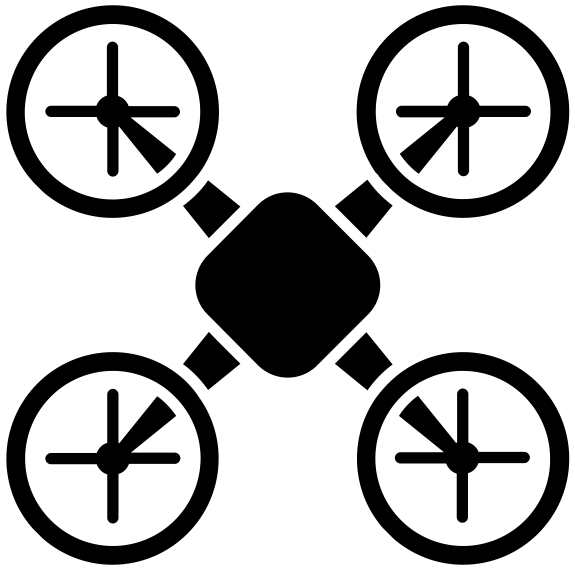
\includegraphics[width=22.5pt,height=22.5pt]{figs/figuras_png_jpg/Drone.png}};
%Image [id:dp4910331142859843] 
\draw (310.67,305) node  {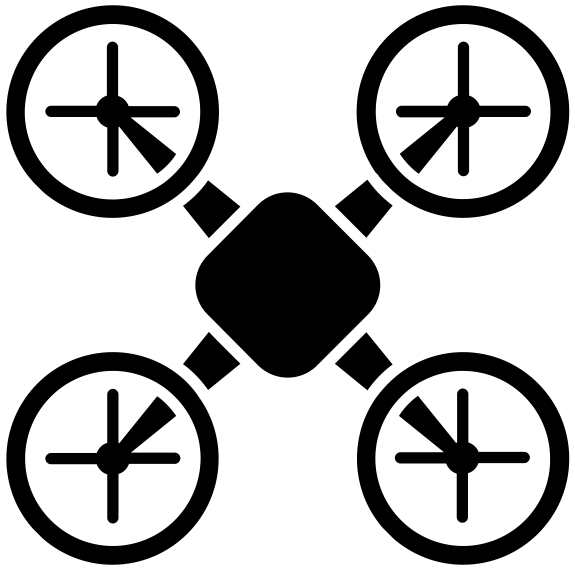
\includegraphics[width=22.5pt,height=22.5pt]{figs/figuras_png_jpg/Drone.png}};
%Image [id:dp9981786601001263] 
\draw (520,323.67) node  {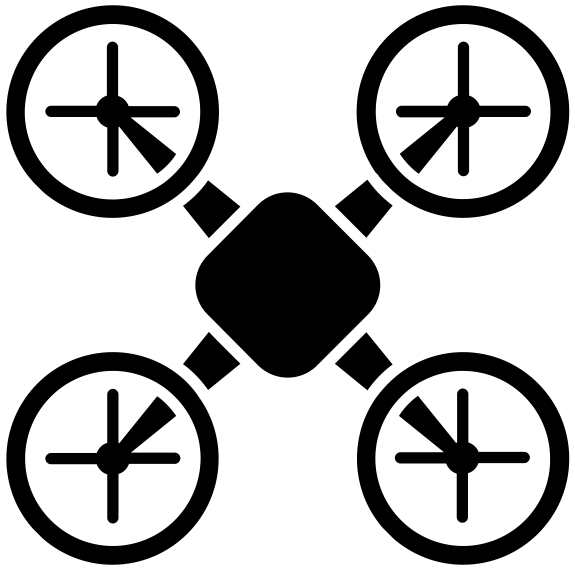
\includegraphics[width=22.5pt,height=22.5pt]{figs/figuras_png_jpg/Drone.png}};
%Image [id:dp557059753604739] 
\draw (56,521) node  {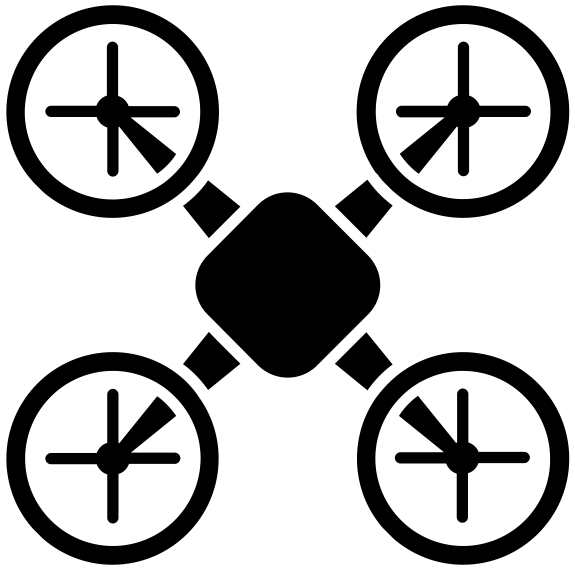
\includegraphics[width=22.5pt,height=22.5pt]{figs/figuras_png_jpg/Drone.png}};
%Image [id:dp529076379845653] 
\draw (351.33,161) node  {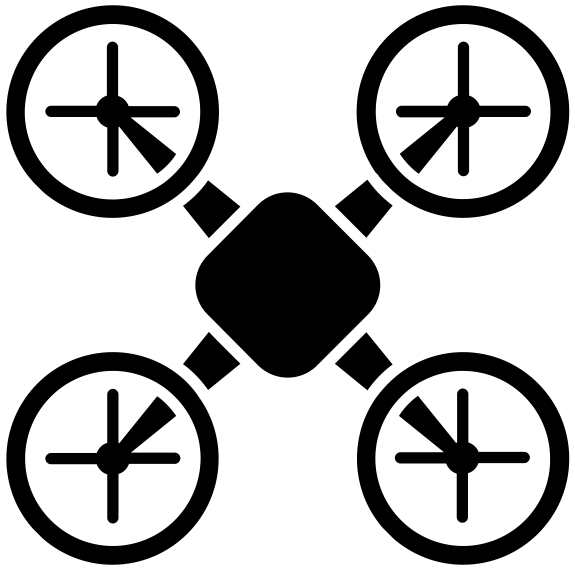
\includegraphics[width=22.5pt,height=22.5pt]{figs/figuras_png_jpg/Drone.png}};


%Straight Lines [id:da21748616719075642] 
\draw [color={rgb, 255:red, 144; green, 19; blue, 254 }  ,draw opacity=1 ] [dash pattern={on 0.84pt off 2.51pt}]  (55.67,390.83) -- (56.33,521.5) ;
%Straight Lines [id:da1928067816905441] 
\draw [color={rgb, 255:red, 144; green, 19; blue, 254 }  ,draw opacity=1 ][fill={rgb, 255:red, 255; green, 255; blue, 255 }  ,fill opacity=1 ] [dash pattern={on 0.84pt off 2.51pt}]  (56.33,521.5) -- (350.33,520.17) ;
%Straight Lines [id:da9351994418641609] 
\draw [color={rgb, 255:red, 144; green, 19; blue, 254 }  ,draw opacity=1 ] [dash pattern={on 0.84pt off 2.51pt}]  (311,305.5) -- (311,390.17) ;
%Straight Lines [id:da3514349689336398] 
\draw [color={rgb, 255:red, 144; green, 19; blue, 254 }  ,draw opacity=1 ] [dash pattern={on 0.84pt off 2.51pt}]  (311,305.5) -- (350.33,305.5) ;
%Straight Lines [id:da702172886065308] 
\draw [color={rgb, 255:red, 144; green, 19; blue, 254 }  ,draw opacity=1 ] [dash pattern={on 0.84pt off 2.51pt}]  (520.33,323.5) -- (520.33,390.17) ;
%Straight Lines [id:da20455880041702157] 
\draw [color={rgb, 255:red, 144; green, 19; blue, 254 }  ,draw opacity=1 ] [dash pattern={on 0.84pt off 2.51pt}]  (520,324.83) -- (350.33,324.83) ;
%Straight Lines [id:da9599452682499601] 
\draw [color={rgb, 255:red, 144; green, 19; blue, 254 }  ,draw opacity=1 ] [dash pattern={on 0.84pt off 2.51pt}]  (515,390.83) -- (515,554.83) ;
%Straight Lines [id:da6739943755378193] 
\draw [color={rgb, 255:red, 144; green, 19; blue, 254 }  ,draw opacity=1 ] [dash pattern={on 0.84pt off 2.51pt}]  (515,554.83) -- (350.33,554.83) ;
%Straight Lines [id:da47528643674774895] 
\draw  [dash pattern={on 0.84pt off 2.51pt}]  (177.33,27.33) -- (256,28) ;
%Shape: Rectangle [id:dp967119633626456] 
\path  [shading=_xegi1ncr4,_lziktnbyh,path fading= _wmear7cqn ,fading transform={xshift=2}] (174,47.5) -- (256,47.5) -- (256,62) -- (174,62) -- cycle ; % for fading 
\draw   (174,47.5) -- (256,47.5) -- (256,62) -- (174,62) -- cycle ; % for border 

%Shape: Axis 2D [id:dp3526983734974858] 
\draw [color={rgb, 255:red, 139; green, 87; blue, 42 }  ,draw opacity=1 ][line width=0.75]  (30,391) -- (670,391)(350,72.24) -- (350,710.63) (663,386) -- (670,391) -- (663,396) (345,79.24) -- (350,72.24) -- (355,79.24) (395,386) -- (395,396)(440,386) -- (440,396)(485,386) -- (485,396)(530,386) -- (530,396)(575,386) -- (575,396)(620,386) -- (620,396)(305,386) -- (305,396)(260,386) -- (260,396)(215,386) -- (215,396)(170,386) -- (170,396)(125,386) -- (125,396)(80,386) -- (80,396)(345,346) -- (355,346)(345,301) -- (355,301)(345,256) -- (355,256)(345,211) -- (355,211)(345,166) -- (355,166)(345,121) -- (355,121)(345,436) -- (355,436)(345,481) -- (355,481)(345,526) -- (355,526)(345,571) -- (355,571)(345,616) -- (355,616)(345,661) -- (355,661) ;
\draw [color={rgb, 255:red, 139; green, 87; blue, 42 }  ,opacity=1 ]  (402,403) node[anchor=east, scale=0.75]{1} (447,403) node[anchor=east, scale=0.75]{2} (492,403) node[anchor=east, scale=0.75]{3} (537,403) node[anchor=east, scale=0.75]{4} (582,403) node[anchor=east, scale=0.75]{5} (627,403) node[anchor=east, scale=0.75]{6} (312,403) node[anchor=east, scale=0.75]{-1} (267,403) node[anchor=east, scale=0.75]{-2} (222,403) node[anchor=east, scale=0.75]{-3} (177,403) node[anchor=east, scale=0.75]{-4} (132,403) node[anchor=east, scale=0.75]{-5} (87,403) node[anchor=east, scale=0.75]{-6} (347,346) node[anchor=east, scale=0.75]{1} (347,301) node[anchor=east, scale=0.75]{2} (347,256) node[anchor=east, scale=0.75]{3} (347,211) node[anchor=east, scale=0.75]{4} (347,166) node[anchor=east, scale=0.75]{5} (347,121) node[anchor=east, scale=0.75]{6} (347,436) node[anchor=east, scale=0.75]{-1} (347,481) node[anchor=east, scale=0.75]{-2} (347,526) node[anchor=east, scale=0.75]{-3} (347,571) node[anchor=east, scale=0.75]{-4} (347,616) node[anchor=east, scale=0.75]{-5} (347,661) node[anchor=east, scale=0.75]{-6} ;
\draw   (35.5,395.67) -- (28.83,390.83) -- (35.5,386) ;
\draw   (355,705.5) -- (350.17,712.17) -- (345.33,705.5) ;
%Straight Lines [id:da9707972416701958] 
\draw [color={rgb, 255:red, 74; green, 144; blue, 226 }  ,draw opacity=1 ] [dash pattern={on 4.5pt off 4.5pt}]  (349,391) -- (130.4,168.43) ;
\draw [shift={(129,167)}, rotate = 405.52] [color={rgb, 255:red, 74; green, 144; blue, 226 }  ,draw opacity=1 ][line width=0.75]    (10.93,-3.29) .. controls (6.95,-1.4) and (3.31,-0.3) .. (0,0) .. controls (3.31,0.3) and (6.95,1.4) .. (10.93,3.29)   ;

% Text Node
\draw (27,367.33) node [anchor=north west][inner sep=0.75pt]   [align=left] {\mbox{-}x};
% Text Node
\draw (648,367) node [anchor=north west][inner sep=0.75pt]   [align=left] {+x};
% Text Node
\draw (356,698.67) node [anchor=north west][inner sep=0.75pt]   [align=left] {\mbox{-}y};
% Text Node
\draw (358,68) node [anchor=north west][inner sep=0.75pt]   [align=left] {+y};
% Text Node
\draw (126.88,164.88) node [anchor=south] [inner sep=0.75pt]  [rotate=-315] [align=left] {{\fontfamily{helvet}\selectfont {\tiny \textcolor[rgb]{0.29,0.56,0.89}{velocidade maxima = 7m/s}}}};
% Text Node
\draw (84.33,47.5) node   [align=left] {\begin{minipage}[lt]{112.42666666666668pt}\setlength\topsep{0pt}
	{\fontfamily{pcr}\selectfont {\footnotesize Areas de velocidade - }}\\{\fontfamily{pcr}\selectfont {\footnotesize Gradiente de velocidade -}}\\
	\end{minipage}};
% Text Node
\draw (293.67,287) node [anchor=south east] [inner sep=0.75pt]   [align=left] {{\fontfamily{pcr}\selectfont {\tiny \textbf{aproximadamente}}}\\\textbf{{\fontfamily{pcr}\selectfont {\tiny x:-0.9m/s ,y:1.9m/s}} \ }};
% Text Node
\draw (521,301.17) node [anchor=south] [inner sep=0.75pt]   [align=left] {{\fontfamily{pcr}\selectfont {\tiny \textbf{aproximadamente}}}\\\textbf{{\fontfamily{pcr}\selectfont {\tiny x:3.8m/s ,y:1.5m/s}} \ }};
% Text Node
\draw (516.33,532.5) node [anchor=south] [inner sep=0.75pt]   [align=left] {{\fontfamily{pcr}\selectfont {\tiny \textbf{aproximadamente}}}\\\textbf{{\fontfamily{pcr}\selectfont {\tiny x:3.75m/s ,y:-3.6m/s}} \ }};
% Text Node
\draw (73,503) node [anchor=south west] [inner sep=0.75pt]   [align=left] {{\fontfamily{pcr}\selectfont {\tiny \textbf{aproximadamente}}}\\\textbf{{\fontfamily{pcr}\selectfont {\tiny x:-6.5m/s ,y:-3.95m/s}} \ }};
% Text Node
\draw (405.67,166.5) node [anchor=south] [inner sep=0.75pt]   [align=left] {{\fontfamily{pcr}\selectfont {\tiny \textbf{aproximadamente}}}\\\textbf{{\fontfamily{pcr}\selectfont {\tiny x:0m/s , y:5m/s}} } };

\draw   (310.22, 520.35) circle [x radius= 5, y radius= 5]   ;
\draw   (225.22, 520.73) circle [x radius= 5, y radius= 5]   ;
\draw   (163.36, 521.01) circle [x radius= 5, y radius= 5]   ;
\draw   (112.44, 521.25) circle [x radius= 5, y radius= 5]   ;
\draw   (62.21, 521.47) circle [x radius= 5, y radius= 5]   ;
\draw   (71, 521.43) circle [x radius= 5, y radius= 5]   ;
\draw   (56.33, 521.5) circle [x radius= 5, y radius= 5]   ;
\draw   (350, 520.17) circle [x radius= 5, y radius= 5]   ;
\end{tikzpicture}



%%Image [id:dp12050943669977343] 
%\draw (514.67,555) node  {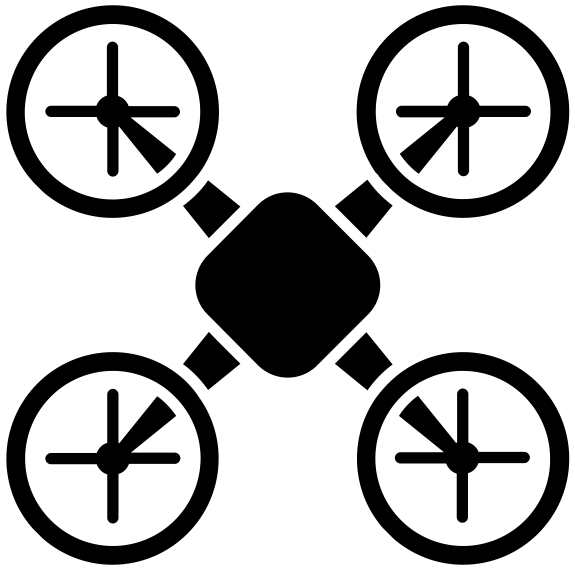
\includegraphics[width=22.5pt,height=22.5pt]{figs/figuras_png_jpg/Drone.png}};
%%Image [id:dp4910331142859843] 
%\draw (310.67,305) node  {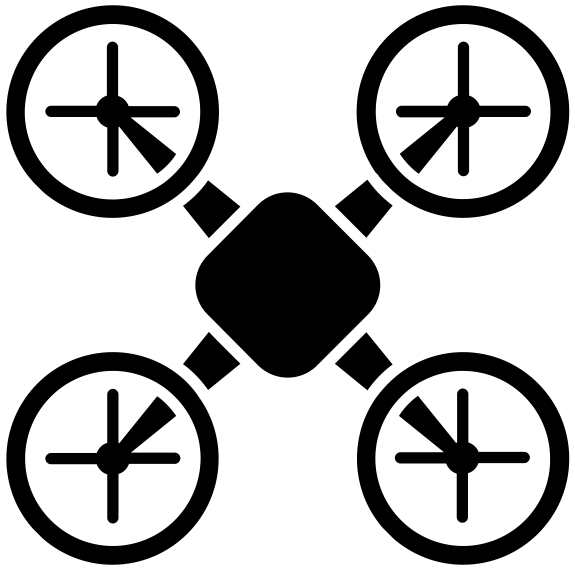
\includegraphics[width=22.5pt,height=22.5pt]{figs/figuras_png_jpg/Drone.png}};
%%Image [id:dp9981786601001263] 
%\draw (520,323.67) node  {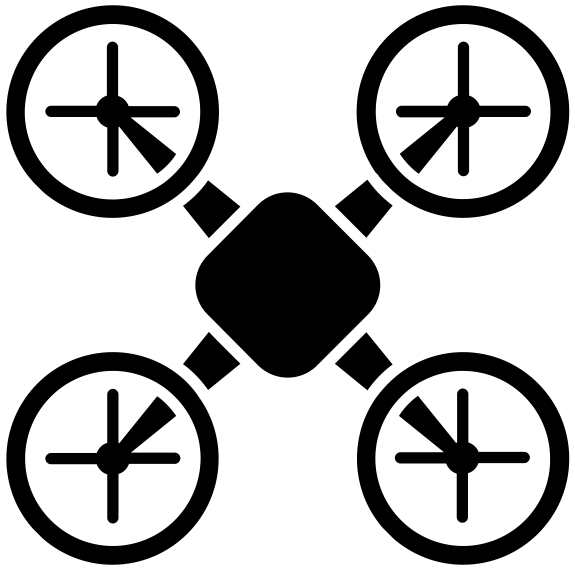
\includegraphics[width=22.5pt,height=22.5pt]{figs/figuras_png_jpg/Drone.png}};
%%Image [id:dp557059753604739] 
%\draw (56,521) node  {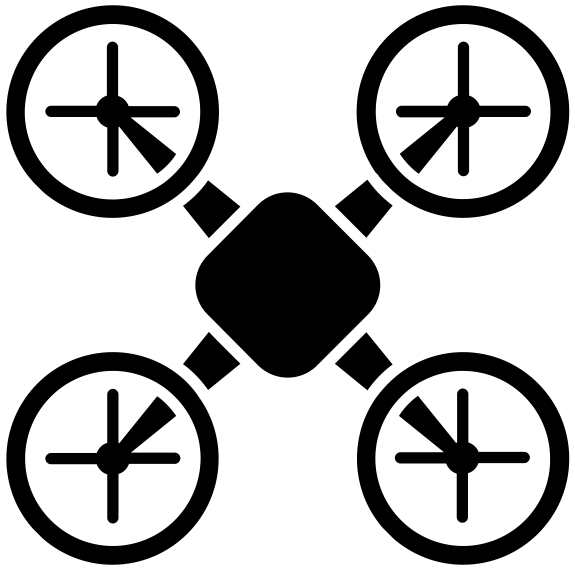
\includegraphics[width=22.5pt,height=22.5pt]{figs/figuras_png_jpg/Drone.png}};
%%Image [id:dp529076379845653] 
%\draw (351.33,161) node  {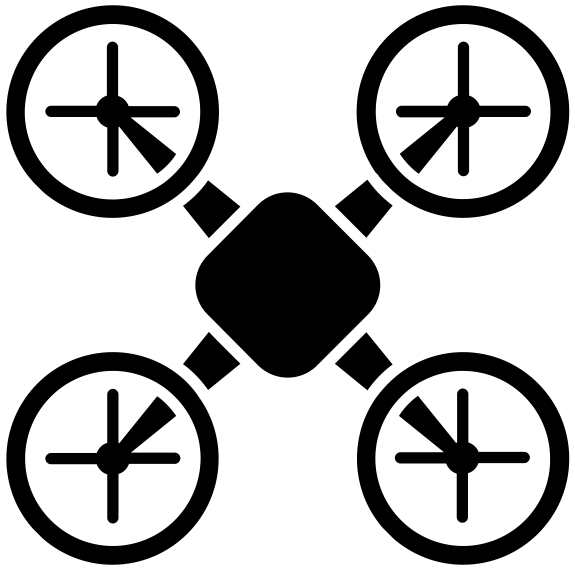
\includegraphics[width=22.5pt,height=22.5pt]{figs/figuras_png_jpg/Drone.png}};

% {figs/figuras_png_jpg/Drone.png}}; \input{figs/svg/Drone.pdf_tex}

%	\def\svgwidth{0.8cm}
%	\input{figs/svg/Drone.pdf_tex}};

%\begin{figure}[htpb]
%	\centering
%	\caption{Simulação real para abstrata}
%	\fontsize{9pt}{12pt}\selectfont
%	%\color{white}
%	\def\svgwidth{15cm}
%	\input{figs/svg/Drone.pdf_tex}
%	\legend{Fonte: a autor.}
%	\label{fig:simul}
%\end{figure}
  	\legend{Fonte: do autor}
\label{fig:teste5}
\end{figure}

\begin{figure}
	\caption{teste}
	% Gradient Info
\tikzset {_q0xe4a8ap/.code = {\pgfsetadditionalshadetransform{ \pgftransformshift{\pgfpoint{0 bp } { 0 bp }  }  \pgftransformscale{1 }  }}}
\pgfdeclareradialshading{_bttg32ha4}{\pgfpoint{0bp}{0bp}}{rgb(0bp)=(0.97,0.91,0.11);
	rgb(0bp)=(0.97,0.91,0.11);
	rgb(25bp)=(0.97,0.91,0.11);
	rgb(400bp)=(0.97,0.91,0.11)}
\tikzset{_2y6lizc3m/.code = {\pgfsetadditionalshadetransform{\pgftransformshift{\pgfpoint{0 bp } { 0 bp }  }  \pgftransformscale{1 } }}}
\pgfdeclareradialshading{_cmven2zpf} { \pgfpoint{0bp} {0bp}} {color(0bp)=(transparent!96);
	color(0bp)=(transparent!96);
	color(25bp)=(transparent!69);
	color(400bp)=(transparent!69)} 
\pgfdeclarefading{_uld39de5b}{\tikz \fill[shading=_cmven2zpf,_2y6lizc3m] (0,0) rectangle (50bp,50bp); } 
\tikzset{every picture/.style={line width=0.75pt}} %set default line width to 0.75pt
       

\begin{tikzpicture}[x=0.75pt,y=0.75pt,yscale=-1,xscale=1]


%Shape: Circle [id:dp12550546475470603] 
\path  [shading=_bttg32ha4,_q0xe4a8ap,path fading= _uld39de5b ,fading transform={xshift=2}] (53,302.75) .. controls (53,145.49) and (180.49,18) .. (337.75,18) .. controls (495.01,18) and (622.5,145.49) .. (622.5,302.75) .. controls (622.5,460.01) and (495.01,587.5) .. (337.75,587.5) .. controls (180.49,587.5) and (53,460.01) .. (53,302.75) -- cycle ;

 % for fading 
%\draw  [dash pattern={on 0.84pt off 2.51pt}] (53,302.75) .. controls (53,145.49) and (180.49,18) .. (337.75,18) .. controls (495.01,18) and (622.5,145.49) .. (622.5,302.75) .. controls (622.5,460.01) and (495.01,587.5) .. (337.75,587.5) .. controls (180.49,587.5) and (53,460.01) .. (53,302.75) -- cycle ; % for border 





\end{tikzpicture}


	\legend{Fonte: do autor}
	\label{fig:teste6}
\end{figure}

\begin{figure}[htpb]
	\centering
	\caption{teste5}
	\fontsize{9pt}{12pt}\selectfont
	%\color{white}
	\def\svgwidth{18cm}
	\input{figs/svg/Drone2.pdf_tex}
	\legend{Fonte: a autor.}
	\label{fig:teste57}
\end{figure}
%-------------------------------------------------------------------------
\begin{figure}
	\caption{teste}
	tikz,border=5mm]{standalone}
\usetikzlibrary{fadings}
\pgfdeclareradialshading{myring}{\pgfpointorigin}
{
	color(0cm)=(transparent!0);
	color(5mm)=(pgftransparent!50);
	color(1cm)=(pgftransparent!100)
}
\pgfdeclarefading{ringo}{\pgfuseshading{myring}}


\begin{tikzpicture}
\filldraw[even odd rule,red ,path fading=ringo] (0,0) circle (16mm) (0,0) circle (2cm);
\filldraw[even odd rule,blue,path fading=ringo] (0,0) circle (3mm) (0,0) circle (0.5cm);
\end{tikzpicture}


	\legend{Fonte: do autor}
	\label{fig:teste7}
\end{figure}% Gradient Info




\begin{figure}
	\caption{teste8}
	% Gradient Info
  
\tikzset {_1nmj4ooki/.code = {\pgfsetadditionalshadetransform{ \pgftransformshift{\pgfpoint{0 bp } { 0 bp }  }  \pgftransformscale{1.14 }  }}}
\pgfdeclareradialshading{_t6d7qbauo}{\pgfpoint{0bp}{0bp}}{rgb(0bp)=(0.97,0.91,0.11);
rgb(0bp)=(0.97,0.91,0.11);
rgb(25bp)=(1,0.92,0);
rgb(400bp)=(1,0.92,0)}
\tikzset{_jedl70pdb/.code = {\pgfsetadditionalshadetransform{\pgftransformshift{\pgfpoint{0 bp } { 0 bp }  }  \pgftransformscale{1.14 } }}}
\pgfdeclareradialshading{_9dwam9ipn} { \pgfpoint{0bp} {0bp}} {color(0bp)=(transparent!100);
color(0bp)=(transparent!100);
color(25bp)=(transparent!0);
color(400bp)=(transparent!0)} 
\pgfdeclarefading{_0k0oruku7}{\tikz \fill[shading=_9dwam9ipn,_jedl70pdb] (0,0) rectangle (50bp,50bp); } 

% Gradient Info
  
\tikzset {_9ie78tr46/.code = {\pgfsetadditionalshadetransform{ \pgftransformshift{\pgfpoint{0 bp } { 0 bp }  }  \pgftransformrotate{0 }  \pgftransformscale{3.6 }  }}}
\pgfdeclarehorizontalshading{_b1j7ieg3b}{150bp}{rgb(0bp)=(0.97,0.91,0.11);
rgb(37.5bp)=(0.97,0.91,0.11);
rgb(62.5bp)=(0.97,0.91,0.11);
rgb(100bp)=(0.97,0.91,0.11)}
\tikzset{_9z21f3uaq/.code = {\pgfsetadditionalshadetransform{\pgftransformshift{\pgfpoint{0 bp } { 0 bp }  }  \pgftransformrotate{0 }  \pgftransformscale{3.6 } }}}
\pgfdeclarehorizontalshading{_bjbtrsbz2} {150bp} {color(0bp)=(transparent!100);
color(37.5bp)=(transparent!100);
color(62.5bp)=(transparent!7);
color(100bp)=(transparent!7) } 
\pgfdeclarefading{_yi0b2856l}{\tikz \fill[shading=_bjbtrsbz2,_9z21f3uaq] (0,0) rectangle (50bp,50bp); } 
\tikzset{every picture/.style={line width=0.75pt}} %set default line width to 0.75pt        

\begin{tikzpicture}[x=0.73pt,y=0.73pt,yscale=-1,xscale=1]
%uncomment if require: \path (0,747); %set diagram left start at 0, and has height of 747

%Flowchart: Connector [id:dp9463721097190696] 
\path  [shading=_t6d7qbauo,_1nmj4ooki,path fading= _0k0oruku7 ,fading transform={xshift=2}] (17,389) .. controls (17,215.03) and (158.03,74) .. (332,74) .. controls (505.97,74) and (647,215.03) .. (647,389) .. controls (647,562.97) and (505.97,704) .. (332,704) .. controls (158.03,704) and (17,562.97) .. (17,389) -- cycle ; % for fading 
 \draw  [color={rgb, 255:red, 155; green, 155; blue, 155 }  ,draw opacity=1 ][dash pattern={on 0.84pt off 2.51pt}] (17,389) .. controls (17,215.03) and (158.03,74) .. (332,74) .. controls (505.97,74) and (647,215.03) .. (647,389) .. controls (647,562.97) and (505.97,704) .. (332,704) .. controls (158.03,704) and (17,562.97) .. (17,389) -- cycle ; % for border 

%Flowchart: Connector [id:dp5881727880187859] 
\draw  [color={rgb, 255:red, 155; green, 155; blue, 155 }  ,draw opacity=1 ][dash pattern={on 0.84pt off 2.51pt}] (241,388.86) .. controls (241.08,339.15) and (281.44,298.92) .. (331.14,299) .. controls (380.85,299.08) and (421.08,339.44) .. (421,389.14) .. controls (420.92,438.85) and (380.56,479.08) .. (330.86,479) .. controls (281.15,478.92) and (240.92,438.56) .. (241,388.86) -- cycle ;
%Flowchart: Connector [id:dp7722946353896842] 
\draw  [color={rgb, 255:red, 155; green, 155; blue, 155 }  ,draw opacity=1 ][dash pattern={on 0.84pt off 2.51pt}] (287,388.92) .. controls (287.04,364.06) and (307.23,343.94) .. (332.08,343.99) .. controls (356.93,344.03) and (377.04,364.22) .. (377,389.08) .. controls (376.96,413.94) and (356.77,434.06) .. (331.92,434.01) .. controls (307.07,433.97) and (286.96,413.78) .. (287,388.92) -- cycle ;
%Flowchart: Connector [id:dp2544406835626385] 
\draw  [color={rgb, 255:red, 155; green, 155; blue, 155 }  ,draw opacity=1 ][dash pattern={on 0.84pt off 2.51pt}] (196,388.79) .. controls (196.12,314.23) and (256.65,253.88) .. (331.21,254) .. controls (405.77,254.12) and (466.12,314.65) .. (466,389.21) .. controls (465.88,463.77) and (405.35,524.12) .. (330.79,524) .. controls (256.23,523.88) and (195.88,463.35) .. (196,388.79) -- cycle ;
%Flowchart: Connector [id:dp06000631406232526] 
\draw  [color={rgb, 255:red, 155; green, 155; blue, 155 }  ,draw opacity=1 ][dash pattern={on 0.84pt off 2.51pt}] (152,388.72) .. controls (152.16,289.31) and (232.87,208.84) .. (332.28,209) .. controls (431.69,209.16) and (512.16,289.87) .. (512,389.28) .. controls (511.84,488.69) and (431.13,569.16) .. (331.72,569) .. controls (232.31,568.84) and (151.84,488.13) .. (152,388.72) -- cycle ;
%Flowchart: Connector [id:dp7137214863827623] 
\draw  [color={rgb, 255:red, 155; green, 155; blue, 155 }  ,draw opacity=1 ][dash pattern={on 0.84pt off 2.51pt}] (106,388.65) .. controls (106.2,261.62) and (207.1,158.81) .. (331.36,159) .. controls (455.63,159.2) and (556.2,262.33) .. (556,389.35) .. controls (555.8,516.38) and (454.9,619.19) .. (330.64,619) .. controls (206.37,618.8) and (105.8,515.67) .. (106,388.65) -- cycle ;
%Flowchart: Connector [id:dp4392817757131624] 
\draw  [color={rgb, 255:red, 155; green, 155; blue, 155 }  ,draw opacity=1 ][dash pattern={on 0.84pt off 2.51pt}] (61,388.58) .. controls (61.23,239.46) and (182.31,118.77) .. (331.42,119) .. controls (480.54,119.23) and (601.23,240.31) .. (601,389.42) .. controls (600.77,538.54) and (479.69,659.23) .. (330.58,659) .. controls (181.46,658.77) and (60.77,537.69) .. (61,388.58) -- cycle ;
%Straight Lines [id:da47528643674774895] 
\draw  [dash pattern={on 0.84pt off 2.51pt}]  (232.33,17.33) -- (311,18) ;
%Shape: Rectangle [id:dp967119633626456] 
\path  [shading=_b1j7ieg3b,_9ie78tr46,path fading= _yi0b2856l ,fading transform={xshift=2}] (231,25.5) -- (313,25.5) -- (313,40) -- (231,40) -- cycle ; % for fading 
 \draw   (231,25.5) -- (313,25.5) -- (313,40) -- (231,40) -- cycle ; % for border 

%Shape: Axis 2D [id:dp3526983734974858] 
\draw [color={rgb, 255:red, 139; green, 87; blue, 42 }  ,draw opacity=1 ][line width=0.75]  (12,389) -- (652,389)(332,70.24) -- (332,708.63) (645,384) -- (652,389) -- (645,394) (327,77.24) -- (332,70.24) -- (337,77.24) (377,384) -- (377,394)(422,384) -- (422,394)(467,384) -- (467,394)(512,384) -- (512,394)(557,384) -- (557,394)(602,384) -- (602,394)(287,384) -- (287,394)(242,384) -- (242,394)(197,384) -- (197,394)(152,384) -- (152,394)(107,384) -- (107,394)(62,384) -- (62,394)(327,344) -- (337,344)(327,299) -- (337,299)(327,254) -- (337,254)(327,209) -- (337,209)(327,164) -- (337,164)(327,119) -- (337,119)(327,434) -- (337,434)(327,479) -- (337,479)(327,524) -- (337,524)(327,569) -- (337,569)(327,614) -- (337,614)(327,659) -- (337,659) ;
\draw [color={rgb, 255:red, 139; green, 87; blue, 42 }  ,opacity=1 ]  (384,401) node[anchor=east, scale=0.75]{1} (429,401) node[anchor=east, scale=0.75]{2} (474,401) node[anchor=east, scale=0.75]{3} (519,401) node[anchor=east, scale=0.75]{4} (564,401) node[anchor=east, scale=0.75]{5} (609,401) node[anchor=east, scale=0.75]{6} (294,401) node[anchor=east, scale=0.75]{-1} (249,401) node[anchor=east, scale=0.75]{-2} (204,401) node[anchor=east, scale=0.75]{-3} (159,401) node[anchor=east, scale=0.75]{-4} (114,401) node[anchor=east, scale=0.75]{-5} (69,401) node[anchor=east, scale=0.75]{-6} (329,344) node[anchor=east, scale=0.75]{1} (329,299) node[anchor=east, scale=0.75]{2} (329,254) node[anchor=east, scale=0.75]{3} (329,209) node[anchor=east, scale=0.75]{4} (329,164) node[anchor=east, scale=0.75]{5} (329,119) node[anchor=east, scale=0.75]{6} (329,434) node[anchor=east, scale=0.75]{-1} (329,479) node[anchor=east, scale=0.75]{-2} (329,524) node[anchor=east, scale=0.75]{-3} (329,569) node[anchor=east, scale=0.75]{-4} (329,614) node[anchor=east, scale=0.75]{-5} (329,659) node[anchor=east, scale=0.75]{-6} ;
\draw   (17.5,393.67) -- (10.83,388.83) -- (17.5,384) ;
\draw   (337,703.5) -- (332.17,710.17) -- (327.33,703.5) ;
%Straight Lines [id:da702172886065308] 
%\draw [color={rgb, 255:red, 144; green, 19; blue, 254 }  ,draw opacity=1 ][line width=1.5]  [dash pattern={on 1.69pt off 2.76pt}]  (502.33,321.5) -- (502.33,388.17) ;
%Straight Lines [id:da20455880041702157] 
%\draw [color={rgb, 255:red, 144; green, 19; blue, 254 }  ,draw opacity=1 ][line width=1.5]  [dash pattern={on 1.69pt off 2.76pt}]  (502,322.83) -- (332.33,322.83) ;
%Straight Lines [id:da9351994418641609] 
%\draw [color={rgb, 255:red, 144; green, 19; blue, 254 }  ,draw opacity=1 ][line width=1.5]  [dash pattern={on 1.69pt off 2.76pt}]  (293,303.5) -- (293,388.17) ;
%Straight Lines [id:da3514349689336398] 
%\draw [color={rgb, 255:red, 144; green, 19; blue, 254 }  ,draw opacity=1 ][line width=1.5]  [dash pattern={on 1.69pt off 2.76pt}]  (293,303.5) -- (332.33,303.5) ;
%Straight Lines [id:da5950502895082348] 
%\draw [color={rgb, 255:red, 189; green, 16; blue, 224 }  ,draw opacity=1 ][line width=1.5]  [dash pattern={on 1.69pt off 2.76pt}]  (38.33,519.5) -- (332.5,518) ;
%Straight Lines [id:da21748616719075642] 
%\draw [color={rgb, 255:red, 144; green, 19; blue, 254 }  ,draw opacity=1 ][line width=1.5]  [dash pattern={on 1.69pt off 2.76pt}]  (37.67,388.83) -- (38.33,519.5) ;
%Straight Lines [id:da6739943755378193] 
%\draw [color={rgb, 255:red, 144; green, 19; blue, 254 }  ,draw opacity=1 ][line width=1.5]  [dash pattern={on 1.69pt off 2.76pt}]  (497,552.83) -- (332.33,552.83) ;
%Straight Lines [id:da9599452682499601] 
%\draw [color={rgb, 255:red, 144; green, 19; blue, 254 }  ,draw opacity=1 ][line width=1.5]  [dash pattern={on 1.69pt off 2.76pt}]  (497,388.83) -- (497,552.83) ;
%Straight Lines [id:da9707972416701958] 
\draw [color={rgb, 255:red, 74; green, 144; blue, 226 }  ,draw opacity=1 ][line width=1.5]  [dash pattern={on 5.63pt off 4.5pt}]  (331,389) -- (113.1,167.14) ;
\draw [shift={(111,165)}, rotate = 405.52] [color={rgb, 255:red, 74; green, 144; blue, 226 }  ,draw opacity=1 ][line width=1.5]    (14.21,-4.28) .. controls (9.04,-1.82) and (4.3,-0.39) .. (0,0) .. controls (4.3,0.39) and (9.04,1.82) .. (14.21,4.28)   ;

%%Image [id:dp4910331142859843] 
%\draw (292.67,302.67) node  {
%\def\svgwidth{1cm}
%\input{{figs/svg/drone3.pdf_tex}}};
%
%	
%%Image [id:dp529076379845653] 
%\draw (331.67,159.67) node {
%\def\svgwidth{1cm}
%\input{{figs/svg/drone3.pdf_tex}}};
%	
%%Image [id:dp557059753604739] 
%\draw (40,519.33) node  {
%\def\svgwidth{1cm}
%\input{{figs/svg/drone3.pdf_tex}}};
%	
%%Image [id:dp9981786601001263] 
%\draw (502.33,323) node  {
%\def\svgwidth{1cm}
%\input{{figs/svg/drone3.pdf_tex}}};
%
%%Image [id:dp12050943669977343] 
%\draw (495.67,551) node  {
%\def\svgwidth{1cm}
%\input{{figs/svg/drone3.pdf_tex}}};	

% Text Node
\draw (10,373.33) node [anchor=north west][inner sep=0.75pt]   [align=left] {\mbox{-}y};
% Text Node
\draw (630,373) node [anchor=north west][inner sep=0.75pt]   [align=left] {+y};
% Text Node
\draw (341,690.67) node [anchor=north west][inner sep=0.75pt]   [align=left] {\mbox{-}x};
% Text Node
\draw (339,80) node [anchor=north west][inner sep=0.75pt]   [align=left] {+x};
% Text Node
\draw (84.88,180.88) node [anchor=south] [inner sep=0.75pt]  [rotate=-315] [align=left] {{\fontfamily{helvet}\selectfont {\tiny \textcolor[rgb]{0.29,0.56,0.89}{velocidade máxima $\displaystyle \eqsim 5m/s$}}}};
% Text Node $\displaystyle a\eqsim b$
\draw (135.83,41.83) node   [align=left] {\begin{minipage}[lt]{156.62666666666667pt}\setlength\topsep{0pt}
{\fontfamily{pcr}\selectfont {\scriptsize Áreas de velocidade - }}\\{\fontfamily{pcr}\selectfont {\scriptsize Gradiente de velocidade -}}\\
\end{minipage}};
% Text Node
%\draw (275.67,285) node [anchor=south east] [inner sep=0.75pt]   [align=left] {{\fontfamily{pcr}\selectfont {\tiny \textbf{aproximadamente}}}\\\textbf{{\fontfamily{pcr}\selectfont {\tiny x:-0.9m/s ,y:1.9m/s}} \ }};
% Text Node
%\draw (503,299.17) node [anchor=south] [inner sep=0.75pt]   [align=left] {{\fontfamily{pcr}\selectfont {\tiny \textbf{aproximadamente}}}\\\textbf{{\fontfamily{pcr}\selectfont {\tiny x:3.8m/s ,y:1.5m/s}} \ }};
% Text Node
%\draw (498.33,530.5) node [anchor=south] [inner sep=0.75pt]   [align=left] {{\fontfamily{pcr}\selectfont {\tiny \textbf{aproximadamente}}}\\\textbf{{\fontfamily{pcr}\selectfont {\tiny x:3.75m/s ,y:-3.6m/s}} \ }};
% Text Node
%\draw (55,501) node [anchor=south west] [inner sep=0.75pt]   [align=left] {{\fontfamily{pcr}\selectfont {\tiny \textbf{aproximadamente}}}\\\textbf{{\fontfamily{pcr}\selectfont {\tiny x:-6.5m/s ,y:-3.95m/s}} \ }};
% Text Node
%\draw (407.67,164.5) node [anchor=south] [inner sep=0.75pt]   [align=left] {{\fontfamily{pcr}\selectfont {\tiny \textbf{aproximadamente}}}\\\textbf{{\fontfamily{pcr}\selectfont {\tiny x:0m/s , y:5m/s}} } };
% Text Node
%\draw (282.67,82.33) node [anchor=north west][inner sep=0.75pt]   [align=left] {\textcolor{olive}{\textbf{Norte}}};
%% Text Node
%\draw (589.33,345.67) node [anchor=north west][inner sep=0.75pt]   [align=left] {\textcolor{olive}{\textbf{Leste}}};
%% Text Node
%\draw (32.67,355) node [anchor=north west][inner sep=0.75pt]   [align=left] {\textcolor{olive}{\textbf{Oeste}}};
%% Text Node
%\draw (297.33,675.67) node [anchor=north west][inner sep=0.75pt]   [align=left] {\textcolor{olive}{\textbf{Sul}}};
% Text Node
%\draw (100,176) node [anchor=north west][inner sep=0.75pt]   [align=left] {\textbf{A}};
%% Text Node
%\draw (557,186) node [anchor=north west][inner sep=0.75pt]   [align=left] {\textbf{B}};
%% Text Node
%\draw (115,597) node [anchor=north west][inner sep=0.75pt]   [align=left] {\textbf{C}};
%% Text Node
%\draw (547,591) node [anchor=north west][inner sep=0.75pt]   [align=left] {\textbf{D}};

%\draw   (310.22, 520.35) circle [x radius= 5, y radius= 5]   ;
%\draw   (225.22, 520.73) circle [x radius= 5, y radius= 5]   ;
%\draw   (163.36, 521.01) circle [x radius= 5, y radius= 5]   ;
%\draw   (112.44, 521.25) circle [x radius= 5, y radius= 5]   ;
%\draw   (62.21, 521.47) circle [x radius= 5, y radius= 5]   ;
%\draw   (71, 521.43) circle [x radius= 5, y radius= 5]   ;
%\draw   (56.33, 521.5) circle [x radius= 5, y radius= 5]   ;
%\draw   (350, 520.17) circle [x radius= 5, y radius= 5]   ;
\end{tikzpicture}


	\legend{Fonte: do autor}
	\label{fig:teste8}
\end{figure}

\begin{figure}
	\caption{teste9}
	% Gradient Info
  
\tikzset {_u2y3p9dde/.code = {\pgfsetadditionalshadetransform{ \pgftransformshift{\pgfpoint{0 bp } { 0 bp }  }  \pgftransformrotate{0 }  \pgftransformscale{4 }  }}}
\pgfdeclarehorizontalshading{_o9uf4r8i7}{150bp}{rgb(0bp)=(0.82,0.01,0.11);
rgb(37.589285714285715bp)=(0.82,0.01,0.11);
rgb(49.64285714285714bp)=(0.82,0.01,0.11);
rgb(62.5bp)=(0.82,0.01,0.11);
rgb(100bp)=(0.82,0.01,0.11)}
\tikzset{_k3xpfmspc/.code = {\pgfsetadditionalshadetransform{\pgftransformshift{\pgfpoint{0 bp } { 0 bp }  }  \pgftransformrotate{0 }  \pgftransformscale{4 } }}}
\pgfdeclarehorizontalshading{_7sidw3eek} {150bp} {color(0bp)=(transparent!0);
color(37.589285714285715bp)=(transparent!0);
color(49.64285714285714bp)=(transparent!100);
color(62.5bp)=(transparent!0);
color(100bp)=(transparent!0) } 
\pgfdeclarefading{_lb6zfszms}{\tikz \fill[shading=_7sidw3eek,_k3xpfmspc] (0,0) rectangle (50bp,50bp); } 

% Gradient Info
  
\tikzset {_ytdjpc7dm/.code = {\pgfsetadditionalshadetransform{ \pgftransformshift{\pgfpoint{0 bp } { 0 bp }  }  \pgftransformrotate{-90 }  \pgftransformscale{4 }  }}}
\pgfdeclarehorizontalshading{_07rypc9bg}{150bp}{rgb(0bp)=(0.49,0.83,0.13);
rgb(37.589285714285715bp)=(0.49,0.83,0.13);
rgb(49.64285714285714bp)=(0.49,0.83,0.13);
rgb(62.5bp)=(0.49,0.83,0.13);
rgb(100bp)=(0.49,0.83,0.13)}
\tikzset{_mgyz19z9a/.code = {\pgfsetadditionalshadetransform{\pgftransformshift{\pgfpoint{0 bp } { 0 bp }  }  \pgftransformrotate{-90 }  \pgftransformscale{4 } }}}
\pgfdeclarehorizontalshading{_7oeqsasgh} {150bp} {color(0bp)=(transparent!0);
color(37.589285714285715bp)=(transparent!0);
color(49.64285714285714bp)=(transparent!100);
color(62.5bp)=(transparent!0);
color(100bp)=(transparent!0) } 
\pgfdeclarefading{_3gin1qm9m}{\tikz \fill[shading=_7oeqsasgh,_mgyz19z9a] (0,0) rectangle (50bp,50bp); } 

% Gradient Info
  
\tikzset {_re24w7kuc/.code = {\pgfsetadditionalshadetransform{ \pgftransformshift{\pgfpoint{0 bp } { 0 bp }  }  \pgftransformrotate{0 }  \pgftransformscale{3.6 }  }}}
\pgfdeclarehorizontalshading{_zliph5uwe}{150bp}{rgb(0bp)=(0.49,0.83,0.13);
rgb(37.5bp)=(0.49,0.83,0.13);
rgb(62.5bp)=(0.49,0.83,0.13);
rgb(100bp)=(0.49,0.83,0.13)}
\tikzset{_uzz9xwq5q/.code = {\pgfsetadditionalshadetransform{\pgftransformshift{\pgfpoint{0 bp } { 0 bp }  }  \pgftransformrotate{0 }  \pgftransformscale{3.6 } }}}
\pgfdeclarehorizontalshading{_njmyxoswn} {150bp} {color(0bp)=(transparent!100);
color(37.5bp)=(transparent!100);
color(62.5bp)=(transparent!14);
color(100bp)=(transparent!14) } 
\pgfdeclarefading{_2l1c9206l}{\tikz \fill[shading=_njmyxoswn,_uzz9xwq5q] (0,0) rectangle (50bp,50bp); } 

% Gradient Info
  
\tikzset {_cibblijk9/.code = {\pgfsetadditionalshadetransform{ \pgftransformshift{\pgfpoint{0 bp } { 0 bp }  }  \pgftransformrotate{0 }  \pgftransformscale{3.6 }  }}}
\pgfdeclarehorizontalshading{_vj1c5txvz}{150bp}{rgb(0bp)=(0.82,0.01,0.11);
rgb(37.5bp)=(0.82,0.01,0.11);
rgb(62.5bp)=(0.82,0.01,0.11);
rgb(100bp)=(0.82,0.01,0.11)}
\tikzset{_i2hou2efn/.code = {\pgfsetadditionalshadetransform{\pgftransformshift{\pgfpoint{0 bp } { 0 bp }  }  \pgftransformrotate{0 }  \pgftransformscale{3.6 } }}}
\pgfdeclarehorizontalshading{_vic7d4zat} {150bp} {color(0bp)=(transparent!100);
color(37.5bp)=(transparent!100);
color(62.5bp)=(transparent!14);
color(100bp)=(transparent!14) } 
\pgfdeclarefading{_lchimy15d}{\tikz \fill[shading=_vic7d4zat,_i2hou2efn] (0,0) rectangle (50bp,50bp); } 
\tikzset{every picture/.style={line width=0.75pt}} %set default line width to 0.75pt        

\begin{tikzpicture}[x=0.75pt,y=0.75pt,yscale=-1,xscale=1]
%uncomment if require: \path (0,747); %set diagram left start at 0, and has height of 747

%Flowchart: Connector [id:dp9463721097190696] 
\path  [shading=_o9uf4r8i7,_u2y3p9dde,path fading= _lb6zfszms ,fading transform={xshift=2}] (17,389) .. controls (17,215.03) and (158.03,74) .. (332,74) .. controls (505.97,74) and (647,215.03) .. (647,389) .. controls (647,562.97) and (505.97,704) .. (332,704) .. controls (158.03,704) and (17,562.97) .. (17,389) -- cycle ; % for fading 
 \draw  [color={rgb, 255:red, 155; green, 155; blue, 155 }  ,draw opacity=1 ][dash pattern={on 0.84pt off 2.51pt}] (17,389) .. controls (17,215.03) and (158.03,74) .. (332,74) .. controls (505.97,74) and (647,215.03) .. (647,389) .. controls (647,562.97) and (505.97,704) .. (332,704) .. controls (158.03,704) and (17,562.97) .. (17,389) -- cycle ; % for border 

%Flowchart: Connector [id:dp03161820752390754] 
\path  [shading=_07rypc9bg,_ytdjpc7dm,path fading= _3gin1qm9m ,fading transform={xshift=2}] (646,389) .. controls (646,562.97) and (504.97,704) .. (331,704) .. controls (157.03,704) and (16,562.97) .. (16,389) .. controls (16,215.03) and (157.03,74) .. (331,74) .. controls (504.97,74) and (646,215.03) .. (646,389) -- cycle ; % for fading 
 \draw  [color={rgb, 255:red, 155; green, 155; blue, 155 }  ,draw opacity=1 ][dash pattern={on 0.84pt off 2.51pt}] (646,389) .. controls (646,562.97) and (504.97,704) .. (331,704) .. controls (157.03,704) and (16,562.97) .. (16,389) .. controls (16,215.03) and (157.03,74) .. (331,74) .. controls (504.97,74) and (646,215.03) .. (646,389) -- cycle ; % for border 

%Flowchart: Connector [id:dp5881727880187859] 
\draw  [color={rgb, 255:red, 155; green, 155; blue, 155 }  ,draw opacity=1 ][dash pattern={on 0.84pt off 2.51pt}] (241,388.86) .. controls (241.08,339.15) and (281.44,298.92) .. (331.14,299) .. controls (380.85,299.08) and (421.08,339.44) .. (421,389.14) .. controls (420.92,438.85) and (380.56,479.08) .. (330.86,479) .. controls (281.15,478.92) and (240.92,438.56) .. (241,388.86) -- cycle ;
%Flowchart: Connector [id:dp7722946353896842] 
\draw  [color={rgb, 255:red, 155; green, 155; blue, 155 }  ,draw opacity=1 ][dash pattern={on 0.84pt off 2.51pt}] (287,388.92) .. controls (287.04,364.06) and (307.23,343.94) .. (332.08,343.99) .. controls (356.93,344.03) and (377.04,364.22) .. (377,389.08) .. controls (376.96,413.94) and (356.77,434.06) .. (331.92,434.01) .. controls (307.07,433.97) and (286.96,413.78) .. (287,388.92) -- cycle ;
%Flowchart: Connector [id:dp2544406835626385] 
\draw  [color={rgb, 255:red, 155; green, 155; blue, 155 }  ,draw opacity=1 ][dash pattern={on 0.84pt off 2.51pt}] (196,388.79) .. controls (196.12,314.23) and (256.65,253.88) .. (331.21,254) .. controls (405.77,254.12) and (466.12,314.65) .. (466,389.21) .. controls (465.88,463.77) and (405.35,524.12) .. (330.79,524) .. controls (256.23,523.88) and (195.88,463.35) .. (196,388.79) -- cycle ;
%Flowchart: Connector [id:dp06000631406232526] 
\draw  [color={rgb, 255:red, 155; green, 155; blue, 155 }  ,draw opacity=1 ][dash pattern={on 0.84pt off 2.51pt}] (152,388.72) .. controls (152.16,289.31) and (232.87,208.84) .. (332.28,209) .. controls (431.69,209.16) and (512.16,289.87) .. (512,389.28) .. controls (511.84,488.69) and (431.13,569.16) .. (331.72,569) .. controls (232.31,568.84) and (151.84,488.13) .. (152,388.72) -- cycle ;
%Flowchart: Connector [id:dp7137214863827623] 
\draw  [color={rgb, 255:red, 155; green, 155; blue, 155 }  ,draw opacity=1 ][dash pattern={on 0.84pt off 2.51pt}] (106,388.65) .. controls (106.2,261.62) and (207.1,158.81) .. (331.36,159) .. controls (455.63,159.2) and (556.2,262.33) .. (556,389.35) .. controls (555.8,516.38) and (454.9,619.19) .. (330.64,619) .. controls (206.37,618.8) and (105.8,515.67) .. (106,388.65) -- cycle ;
%Flowchart: Connector [id:dp4392817757131624] 
\draw  [color={rgb, 255:red, 155; green, 155; blue, 155 }  ,draw opacity=1 ][dash pattern={on 0.84pt off 2.51pt}] (61,388.58) .. controls (61.23,239.46) and (182.31,118.77) .. (331.42,119) .. controls (480.54,119.23) and (601.23,240.31) .. (601,389.42) .. controls (600.77,538.54) and (479.69,659.23) .. (330.58,659) .. controls (181.46,658.77) and (60.77,537.69) .. (61,388.58) -- cycle ;
%Straight Lines [id:da47528643674774895] 
\draw  [dash pattern={on 0.84pt off 2.51pt}]  (232.33,17.33) -- (311,18) ;
%Shape: Rectangle [id:dp967119633626456] 
\path  [shading=_zliph5uwe,_re24w7kuc,path fading= _2l1c9206l ,fading transform={xshift=2}] (231,25.5) -- (313,25.5) -- (313,40) -- (231,40) -- cycle ; % for fading 
 \draw   (231,25.5) -- (313,25.5) -- (313,40) -- (231,40) -- cycle ; % for border 

%Shape: Axis 2D [id:dp3526983734974858] 
\draw [color={rgb, 255:red, 139; green, 87; blue, 42 }  ,draw opacity=1 ][line width=0.75]  (12,389) -- (652,389)(332,70.24) -- (332,708.63) (645,384) -- (652,389) -- (645,394) (327,77.24) -- (332,70.24) -- (337,77.24) (377,384) -- (377,394)(422,384) -- (422,394)(467,384) -- (467,394)(512,384) -- (512,394)(557,384) -- (557,394)(602,384) -- (602,394)(287,384) -- (287,394)(242,384) -- (242,394)(197,384) -- (197,394)(152,384) -- (152,394)(107,384) -- (107,394)(62,384) -- (62,394)(327,344) -- (337,344)(327,299) -- (337,299)(327,254) -- (337,254)(327,209) -- (337,209)(327,164) -- (337,164)(327,119) -- (337,119)(327,434) -- (337,434)(327,479) -- (337,479)(327,524) -- (337,524)(327,569) -- (337,569)(327,614) -- (337,614)(327,659) -- (337,659) ;
\draw [color={rgb, 255:red, 139; green, 87; blue, 42 }  ,opacity=1 ]  (384,401) node[anchor=east, scale=0.75]{1} (429,401) node[anchor=east, scale=0.75]{2} (474,401) node[anchor=east, scale=0.75]{3} (519,401) node[anchor=east, scale=0.75]{4} (564,401) node[anchor=east, scale=0.75]{5} (609,401) node[anchor=east, scale=0.75]{6} (294,401) node[anchor=east, scale=0.75]{-1} (249,401) node[anchor=east, scale=0.75]{-2} (204,401) node[anchor=east, scale=0.75]{-3} (159,401) node[anchor=east, scale=0.75]{-4} (114,401) node[anchor=east, scale=0.75]{-5} (69,401) node[anchor=east, scale=0.75]{-6} (329,344) node[anchor=east, scale=0.75]{1} (329,299) node[anchor=east, scale=0.75]{2} (329,254) node[anchor=east, scale=0.75]{3} (329,209) node[anchor=east, scale=0.75]{4} (329,164) node[anchor=east, scale=0.75]{5} (329,119) node[anchor=east, scale=0.75]{6} (329,434) node[anchor=east, scale=0.75]{-1} (329,479) node[anchor=east, scale=0.75]{-2} (329,524) node[anchor=east, scale=0.75]{-3} (329,569) node[anchor=east, scale=0.75]{-4} (329,614) node[anchor=east, scale=0.75]{-5} (329,659) node[anchor=east, scale=0.75]{-6} ;
\draw   (17.5,393.67) -- (10.83,388.83) -- (17.5,384) ;
\draw   (337,703.5) -- (332.17,710.17) -- (327.33,703.5) ;
%Shape: Rectangle [id:dp24950383943336263] 
\path  [shading=_vj1c5txvz,_cibblijk9,path fading= _lchimy15d ,fading transform={xshift=2}] (231,47) -- (313,47) -- (313,61.5) -- (231,61.5) -- cycle ; % for fading 
 \draw   (231,47) -- (313,47) -- (313,61.5) -- (231,61.5) -- cycle ; % for border 

%Straight Lines [id:da702172886065308] 
\draw [color={rgb, 255:red, 144; green, 19; blue, 254 }  ,draw opacity=1 ][line width=1.5]  [dash pattern={on 1.69pt off 2.76pt}]  (502.33,321.5) -- (502.33,388.17) ;
%Straight Lines [id:da20455880041702157] 
\draw [color={rgb, 255:red, 144; green, 19; blue, 254 }  ,draw opacity=1 ][line width=1.5]  [dash pattern={on 1.69pt off 2.76pt}]  (502,322.83) -- (332.33,322.83) ;
%Straight Lines [id:da9351994418641609] 
\draw [color={rgb, 255:red, 144; green, 19; blue, 254 }  ,draw opacity=1 ][line width=1.5]  [dash pattern={on 1.69pt off 2.76pt}]  (293,303.5) -- (293,388.17) ;
%Straight Lines [id:da3514349689336398] 
\draw [color={rgb, 255:red, 144; green, 19; blue, 254 }  ,draw opacity=1 ][line width=1.5]  [dash pattern={on 1.69pt off 2.76pt}]  (293,303.5) -- (332.33,303.5) ;
%Straight Lines [id:da5950502895082348] 
\draw [color={rgb, 255:red, 189; green, 16; blue, 224 }  ,draw opacity=1 ][line width=1.5]  [dash pattern={on 1.69pt off 2.76pt}]  (38.33,519.5) -- (332.5,518) ;
%Straight Lines [id:da21748616719075642] 
\draw [color={rgb, 255:red, 144; green, 19; blue, 254 }  ,draw opacity=1 ][line width=1.5]  [dash pattern={on 1.69pt off 2.76pt}]  (37.67,388.83) -- (38.33,519.5) ;
%Straight Lines [id:da6739943755378193] 
\draw [color={rgb, 255:red, 144; green, 19; blue, 254 }  ,draw opacity=1 ][line width=1.5]  [dash pattern={on 1.69pt off 2.76pt}]  (497,552.83) -- (332.33,552.83) ;
%Straight Lines [id:da9599452682499601] 
\draw [color={rgb, 255:red, 144; green, 19; blue, 254 }  ,draw opacity=1 ][line width=1.5]  [dash pattern={on 1.69pt off 2.76pt}]  (497,388.83) -- (497,552.83) ;
%Straight Lines [id:da9707972416701958] 
\draw [color={rgb, 255:red, 74; green, 144; blue, 226 }  ,draw opacity=1 ][line width=1.5]  [dash pattern={on 5.63pt off 4.5pt}]  (331,389) -- (113.1,167.14) ;
\draw [shift={(111,165)}, rotate = 405.52] [color={rgb, 255:red, 74; green, 144; blue, 226 }  ,draw opacity=1 ][line width=1.5]    (14.21,-4.28) .. controls (9.04,-1.82) and (4.3,-0.39) .. (0,0) .. controls (4.3,0.39) and (9.04,1.82) .. (14.21,4.28)   ;

%Image [id:dp4910331142859843] 
%\draw (292.67,302.67) node  {\includegraphics[width=22.5pt,height=22.5pt]{6025c54d-4c76-4719-8b35-c28b7f17b685}};
%Image [id:dp529076379845653] 
%\draw (331.67,159.67) node  {\includegraphics[width=22.5pt,height=22.5pt]{6025c54d-4c76-4719-8b35-c28b7f17b685}};
%Image [id:dp557059753604739] 
%\draw (40,519.33) node  {\includegraphics[width=22.5pt,height=22.5pt]{6025c54d-4c76-4719-8b35-c28b7f17b685}};
%Image [id:dp9981786601001263] 
%\draw (502.33,323) node  {\includegraphics[width=22.5pt,height=22.5pt]{6025c54d-4c76-4719-8b35-c28b7f17b685}};
%Image [id:dp12050943669977343] 
%\draw (495.67,551) node  {\includegraphics[width=22.5pt,height=22.5pt]{6025c54d-4c76-4719-8b35-c28b7f17b685}};

% Text Node
\draw (10,373.33) node [anchor=north west][inner sep=0.75pt]   [align=left] {\mbox{-}x};
% Text Node
\draw (630,373) node [anchor=north west][inner sep=0.75pt]   [align=left] {+x};
% Text Node
\draw (339,707.67) node [anchor=north west][inner sep=0.75pt]   [align=left] {\mbox{-}y};
% Text Node
\draw (339,80) node [anchor=north west][inner sep=0.75pt]   [align=left] {+y};
% Text Node
\draw (84.88,180.88) node [anchor=south] [inner sep=0.75pt]  [rotate=-315] [align=left] {{\fontfamily{helvet}\selectfont {\tiny \textcolor[rgb]{0.29,0.56,0.89}{velocidade máxima = 7m/s}}}};
% Text Node
\draw (115.83,41.83) node   [align=left] {\begin{minipage}[lt]{156.62666666666667pt}\setlength\topsep{0pt}
{\fontfamily{pcr}\selectfont {\scriptsize Áreas de velocidade - }}\\{\fontfamily{pcr}\selectfont {\scriptsize Gradiente de velocidade em y-}}\\{\fontfamily{pcr}\selectfont {\scriptsize Gradiente de velocidade em x-}}\\
\end{minipage}};
% Text Node
\draw (275.67,285) node [anchor=south east] [inner sep=0.75pt]   [align=left] {{\fontfamily{pcr}\selectfont {\tiny \textbf{aproximadamente}}}\\\textbf{{\fontfamily{pcr}\selectfont {\tiny x:-0.9m/s ,y:1.9m/s}} \ }};
% Text Node
\draw (503,299.17) node [anchor=south] [inner sep=0.75pt]   [align=left] {{\fontfamily{pcr}\selectfont {\tiny \textbf{aproximadamente}}}\\\textbf{{\fontfamily{pcr}\selectfont {\tiny x:3.8m/s ,y:1.5m/s}} \ }};
% Text Node
\draw (498.33,530.5) node [anchor=south] [inner sep=0.75pt]   [align=left] {{\fontfamily{pcr}\selectfont {\tiny \textbf{aproximadamente}}}\\\textbf{{\fontfamily{pcr}\selectfont {\tiny x:3.75m/s ,y:-3.6m/s}} \ }};
% Text Node
\draw (55,501) node [anchor=south west] [inner sep=0.75pt]   [align=left] {{\fontfamily{pcr}\selectfont {\tiny \textbf{aproximadamente}}}\\\textbf{{\fontfamily{pcr}\selectfont {\tiny x:-6.5m/s ,y:-3.95m/s}} \ }};
% Text Node
\draw (387.67,164.5) node [anchor=south] [inner sep=0.75pt]   [align=left] {{\fontfamily{pcr}\selectfont {\tiny \textbf{aproximadamente}}}\\\textbf{{\fontfamily{pcr}\selectfont {\tiny x:0m/s , y:5m/s}} } };

% Text Node
\draw (100,176) node [anchor=north west][inner sep=0.75pt]   [align=left] {\textbf{A}};
% Text Node
\draw (557,186) node [anchor=north west][inner sep=0.75pt]   [align=left] {\textbf{B}};
% Text Node
\draw (115,597) node [anchor=north west][inner sep=0.75pt]   [align=left] {\textbf{C}};
% Text Node
\draw (547,591) node [anchor=north west][inner sep=0.75pt]   [align=left] {\textbf{D}};

% Text Node
\draw (282.67,82.33) node [anchor=north west][inner sep=0.75pt]   [align=left] {\textcolor[rgb]{1,1,1}{Norte}};
% Text Node
\draw (589.33,345.67) node [anchor=north west][inner sep=0.75pt]   [align=left] {\textcolor[rgb]{1,1,1}{Leste}};
% Text Node
\draw (32.67,355) node [anchor=north west][inner sep=0.75pt]   [align=left] {\textcolor[rgb]{1,1,1}{Oeste}};
% Text Node
\draw (297.33,675.67) node [anchor=north west][inner sep=0.75pt]   [align=left] {\textcolor[rgb]{1,1,1}{Sul}};

\draw   (310.22, 520.35) circle [x radius= 5, y radius= 5]   ;
\draw   (225.22, 520.73) circle [x radius= 5, y radius= 5]   ;
\draw   (163.36, 521.01) circle [x radius= 5, y radius= 5]   ;
\draw   (112.44, 521.25) circle [x radius= 5, y radius= 5]   ;
\draw   (62.21, 521.47) circle [x radius= 5, y radius= 5]   ;
\draw   (71, 521.43) circle [x radius= 5, y radius= 5]   ;
\draw   (56.33, 521.5) circle [x radius= 5, y radius= 5]   ;
\draw   (350, 520.17) circle [x radius= 5, y radius= 5]   ;
\end{tikzpicture}

	\legend{Fonte: do autor}
	\label{fig:teste9}
\end{figure}
%-----------------------------------------------------------------------
\subsection{Simulações com Hardware}



\subsection{Fluxogramas dos Protótipos}

